% Options for packages loaded elsewhere
\PassOptionsToPackage{unicode}{hyperref}
\PassOptionsToPackage{hyphens}{url}
%
\documentclass[
]{article}
\title{Decision Analysis - Bayesian Networks}
\author{Author: Can Aytöre}
\date{Last Update: 2022-02-20}

\usepackage{amsmath,amssymb}
\usepackage{lmodern}
\usepackage{iftex}
\ifPDFTeX
  \usepackage[T1]{fontenc}
  \usepackage[utf8]{inputenc}
  \usepackage{textcomp} % provide euro and other symbols
\else % if luatex or xetex
  \usepackage{unicode-math}
  \defaultfontfeatures{Scale=MatchLowercase}
  \defaultfontfeatures[\rmfamily]{Ligatures=TeX,Scale=1}
\fi
% Use upquote if available, for straight quotes in verbatim environments
\IfFileExists{upquote.sty}{\usepackage{upquote}}{}
\IfFileExists{microtype.sty}{% use microtype if available
  \usepackage[]{microtype}
  \UseMicrotypeSet[protrusion]{basicmath} % disable protrusion for tt fonts
}{}
\makeatletter
\@ifundefined{KOMAClassName}{% if non-KOMA class
  \IfFileExists{parskip.sty}{%
    \usepackage{parskip}
  }{% else
    \setlength{\parindent}{0pt}
    \setlength{\parskip}{6pt plus 2pt minus 1pt}}
}{% if KOMA class
  \KOMAoptions{parskip=half}}
\makeatother
\usepackage{xcolor}
\IfFileExists{xurl.sty}{\usepackage{xurl}}{} % add URL line breaks if available
\IfFileExists{bookmark.sty}{\usepackage{bookmark}}{\usepackage{hyperref}}
\hypersetup{
  pdftitle={Decision Analysis - Bayesian Networks},
  pdfauthor={Author: Can Aytöre},
  hidelinks,
  pdfcreator={LaTeX via pandoc}}
\urlstyle{same} % disable monospaced font for URLs
\usepackage[margin=1in]{geometry}
\usepackage{color}
\usepackage{fancyvrb}
\newcommand{\VerbBar}{|}
\newcommand{\VERB}{\Verb[commandchars=\\\{\}]}
\DefineVerbatimEnvironment{Highlighting}{Verbatim}{commandchars=\\\{\}}
% Add ',fontsize=\small' for more characters per line
\usepackage{framed}
\definecolor{shadecolor}{RGB}{248,248,248}
\newenvironment{Shaded}{\begin{snugshade}}{\end{snugshade}}
\newcommand{\AlertTok}[1]{\textcolor[rgb]{0.94,0.16,0.16}{#1}}
\newcommand{\AnnotationTok}[1]{\textcolor[rgb]{0.56,0.35,0.01}{\textbf{\textit{#1}}}}
\newcommand{\AttributeTok}[1]{\textcolor[rgb]{0.77,0.63,0.00}{#1}}
\newcommand{\BaseNTok}[1]{\textcolor[rgb]{0.00,0.00,0.81}{#1}}
\newcommand{\BuiltInTok}[1]{#1}
\newcommand{\CharTok}[1]{\textcolor[rgb]{0.31,0.60,0.02}{#1}}
\newcommand{\CommentTok}[1]{\textcolor[rgb]{0.56,0.35,0.01}{\textit{#1}}}
\newcommand{\CommentVarTok}[1]{\textcolor[rgb]{0.56,0.35,0.01}{\textbf{\textit{#1}}}}
\newcommand{\ConstantTok}[1]{\textcolor[rgb]{0.00,0.00,0.00}{#1}}
\newcommand{\ControlFlowTok}[1]{\textcolor[rgb]{0.13,0.29,0.53}{\textbf{#1}}}
\newcommand{\DataTypeTok}[1]{\textcolor[rgb]{0.13,0.29,0.53}{#1}}
\newcommand{\DecValTok}[1]{\textcolor[rgb]{0.00,0.00,0.81}{#1}}
\newcommand{\DocumentationTok}[1]{\textcolor[rgb]{0.56,0.35,0.01}{\textbf{\textit{#1}}}}
\newcommand{\ErrorTok}[1]{\textcolor[rgb]{0.64,0.00,0.00}{\textbf{#1}}}
\newcommand{\ExtensionTok}[1]{#1}
\newcommand{\FloatTok}[1]{\textcolor[rgb]{0.00,0.00,0.81}{#1}}
\newcommand{\FunctionTok}[1]{\textcolor[rgb]{0.00,0.00,0.00}{#1}}
\newcommand{\ImportTok}[1]{#1}
\newcommand{\InformationTok}[1]{\textcolor[rgb]{0.56,0.35,0.01}{\textbf{\textit{#1}}}}
\newcommand{\KeywordTok}[1]{\textcolor[rgb]{0.13,0.29,0.53}{\textbf{#1}}}
\newcommand{\NormalTok}[1]{#1}
\newcommand{\OperatorTok}[1]{\textcolor[rgb]{0.81,0.36,0.00}{\textbf{#1}}}
\newcommand{\OtherTok}[1]{\textcolor[rgb]{0.56,0.35,0.01}{#1}}
\newcommand{\PreprocessorTok}[1]{\textcolor[rgb]{0.56,0.35,0.01}{\textit{#1}}}
\newcommand{\RegionMarkerTok}[1]{#1}
\newcommand{\SpecialCharTok}[1]{\textcolor[rgb]{0.00,0.00,0.00}{#1}}
\newcommand{\SpecialStringTok}[1]{\textcolor[rgb]{0.31,0.60,0.02}{#1}}
\newcommand{\StringTok}[1]{\textcolor[rgb]{0.31,0.60,0.02}{#1}}
\newcommand{\VariableTok}[1]{\textcolor[rgb]{0.00,0.00,0.00}{#1}}
\newcommand{\VerbatimStringTok}[1]{\textcolor[rgb]{0.31,0.60,0.02}{#1}}
\newcommand{\WarningTok}[1]{\textcolor[rgb]{0.56,0.35,0.01}{\textbf{\textit{#1}}}}
\usepackage{longtable,booktabs,array}
\usepackage{calc} % for calculating minipage widths
% Correct order of tables after \paragraph or \subparagraph
\usepackage{etoolbox}
\makeatletter
\patchcmd\longtable{\par}{\if@noskipsec\mbox{}\fi\par}{}{}
\makeatother
% Allow footnotes in longtable head/foot
\IfFileExists{footnotehyper.sty}{\usepackage{footnotehyper}}{\usepackage{footnote}}
\makesavenoteenv{longtable}
\usepackage{graphicx}
\makeatletter
\def\maxwidth{\ifdim\Gin@nat@width>\linewidth\linewidth\else\Gin@nat@width\fi}
\def\maxheight{\ifdim\Gin@nat@height>\textheight\textheight\else\Gin@nat@height\fi}
\makeatother
% Scale images if necessary, so that they will not overflow the page
% margins by default, and it is still possible to overwrite the defaults
% using explicit options in \includegraphics[width, height, ...]{}
\setkeys{Gin}{width=\maxwidth,height=\maxheight,keepaspectratio}
% Set default figure placement to htbp
\makeatletter
\def\fps@figure{htbp}
\makeatother
\setlength{\emergencystretch}{3em} % prevent overfull lines
\providecommand{\tightlist}{%
  \setlength{\itemsep}{0pt}\setlength{\parskip}{0pt}}
\setcounter{secnumdepth}{5}
\ifLuaTeX
  \usepackage{selnolig}  % disable illegal ligatures
\fi
\usepackage[]{natbib}
\bibliographystyle{plainnat}

\begin{document}
\maketitle

{
\setcounter{tocdepth}{2}
\tableofcontents
}
\hypertarget{introduction}{%
\section{Introduction}\label{introduction}}

\hypertarget{aim}{%
\subsection{Aim}\label{aim}}

\hypertarget{motivation}{%
\subsection{Motivation}\label{motivation}}

\begin{itemize}
\tightlist
\item
  We have an understanding of BNs as graphical models representing probability distributions.
\item
  What does that imply in terms of the underlying probability distribution?
\item
  What happens if a probability distribution factorizes with respect to a graph?
\item
  What kind of computations can we make on BNs?
\item
  What kind of questions can we answer using (quantified) BNs?
\end{itemize}

\hypertarget{getting-started-with}{%
\section{Getting Started with \ldots{}}\label{getting-started-with}}

\hypertarget{what-is-bn}{%
\subsection{What is BN?}\label{what-is-bn}}

A Probabilistic Network (aka causal graph, Bayesian belief network, etc.) is a graphical representation of a \textbf{joint probability distribution}.

\hypertarget{running-example-is-the-family-out}{%
\subsection{Running Example: ``Is the Family Out?''}\label{running-example-is-the-family-out}}

When Mr.~West goes home at night, he wants to know if his family is home before trying the doors (maybe because the most convenient door to enter is double locked when nobody is home.) Often, when Mrs.~West leaves the house, she turns on an outdoor light. However, she sometimes turns on this light if she is expecting a guest. Also (and of course!) the Wests have a dog. When nobody is home, the dog is put in the backyard. The same is true if the dog has bowel troubles. Finally, if the dog is in the backyard, Mr.~West will probably hear her barking (or what he thinks is her barking), but sometimes he can be confused by other dogs barking.

\begin{Shaded}
\begin{Highlighting}[]
\NormalTok{fo.data }\OtherTok{\textless{}{-}} \FunctionTok{readRDS}\NormalTok{(}\FunctionTok{url}\NormalTok{(}\StringTok{"https://github.com/canaytore/bayesian{-}networks/raw/main/data/fo\_data.rds"}\NormalTok{)) }\CommentTok{\#fo.data is imported}
\FunctionTok{head}\NormalTok{(fo.data)}
\end{Highlighting}
\end{Shaded}

\begin{verbatim}
##    B   D     F   H     L
## 1 NO  IN FALSE  NO FALSE
## 2 NO OUT  TRUE YES FALSE
## 3 NO  IN FALSE  NO FALSE
## 4 NO OUT  TRUE  NO FALSE
## 5 NO OUT FALSE YES FALSE
## 6 NO  IN  TRUE  NO  TRUE
\end{verbatim}

\begin{Shaded}
\begin{Highlighting}[]
\FunctionTok{library}\NormalTok{(bnlearn)}
\FunctionTok{library}\NormalTok{(gRain)}
\FunctionTok{library}\NormalTok{(ggplot2)}

\NormalTok{fo.dag }\OtherTok{\textless{}{-}} \FunctionTok{model2network}\NormalTok{(}\StringTok{"[F][B][L|F][D|F:B][H|D]"}\NormalTok{) }\CommentTok{\#Family{-}out network is created}
\FunctionTok{graphviz.plot}\NormalTok{(fo.dag)}
\end{Highlighting}
\end{Shaded}

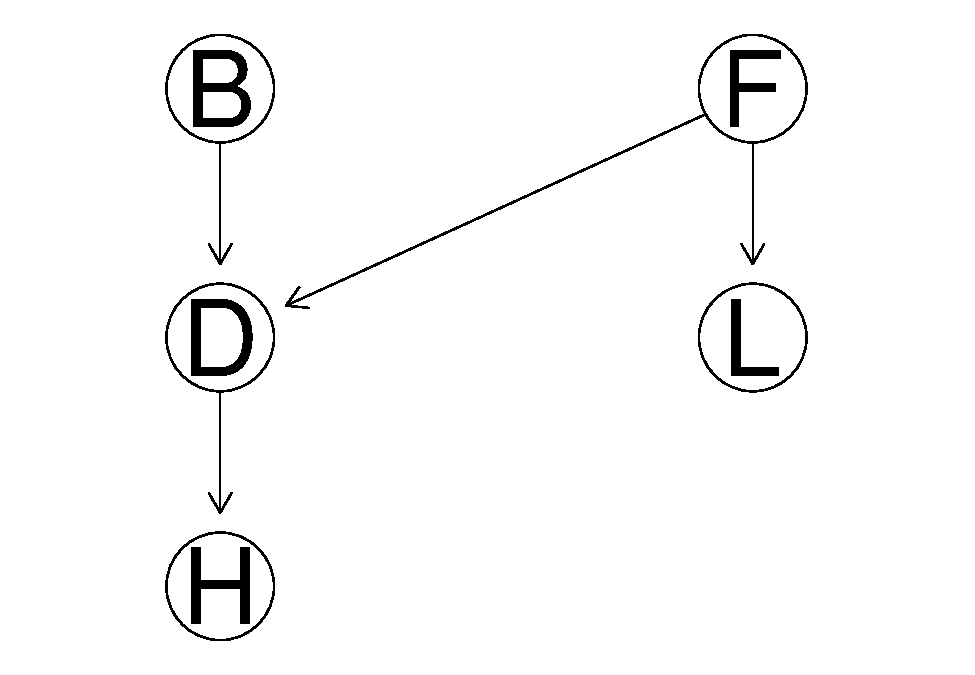
\includegraphics{bayesian_networks_files/figure-latex/unnamed-chunk-2-1.pdf}

Each iteration results will be collected in following arrays.

\begin{Shaded}
\begin{Highlighting}[]
\CommentTok{\#First case: P(F=TRUE) }
\NormalTok{first.mle }\OtherTok{\textless{}{-}} \FunctionTok{array}\NormalTok{(}\AttributeTok{dim =} \DecValTok{20}\NormalTok{)}
\NormalTok{first.bayes }\OtherTok{\textless{}{-}} \FunctionTok{array}\NormalTok{(}\AttributeTok{dim =} \DecValTok{20}\NormalTok{)}

\CommentTok{\#Second case: P(D=OUT | B=YES, F=TRUE)}
\NormalTok{second.mle }\OtherTok{\textless{}{-}} \FunctionTok{array}\NormalTok{(}\AttributeTok{dim =} \DecValTok{20}\NormalTok{)}
\NormalTok{second.bayes }\OtherTok{\textless{}{-}} \FunctionTok{array}\NormalTok{(}\AttributeTok{dim =} \DecValTok{20}\NormalTok{)}
\end{Highlighting}
\end{Shaded}

Now that we have a model ( fo.dag ) and data ( fo.data )
We can learn the conditional probability tables (parameters) using the bn.fit function which implements the maximum likelihood maximization and a Bayesian method to learn parameters.

\begin{Shaded}
\begin{Highlighting}[]
\ControlFlowTok{for}\NormalTok{(i }\ControlFlowTok{in} \DecValTok{1}\SpecialCharTok{:}\DecValTok{20}\NormalTok{)\{}
  \CommentTok{\#P(F=TRUE) using mle:}
\NormalTok{  first.mle[i] }\OtherTok{\textless{}{-}} \FunctionTok{bn.fit}\NormalTok{(fo.dag, fo.data[}\DecValTok{1}\SpecialCharTok{:}\NormalTok{(}\DecValTok{500}\SpecialCharTok{*}\NormalTok{i),])}\SpecialCharTok{$}\NormalTok{F}\SpecialCharTok{$}\NormalTok{prob[}\StringTok{"TRUE"}\NormalTok{]}
  \CommentTok{\#P(F=TRUE) using bayes:}
\NormalTok{  first.bayes[i] }\OtherTok{\textless{}{-}} \FunctionTok{bn.fit}\NormalTok{(fo.dag, fo.data[}\DecValTok{1}\SpecialCharTok{:}\NormalTok{(}\DecValTok{500}\SpecialCharTok{*}\NormalTok{i),], }\AttributeTok{method =} \StringTok{"bayes"}\NormalTok{, }\AttributeTok{iss=}\DecValTok{10}\NormalTok{)}\SpecialCharTok{$}\NormalTok{F}\SpecialCharTok{$}\NormalTok{prob[}\StringTok{"TRUE"}\NormalTok{]}
  
  \CommentTok{\#P(D=OUT | B=YES, F=TRUE) using mle:}
\NormalTok{  second.mle[i] }\OtherTok{\textless{}{-}} \FunctionTok{bn.fit}\NormalTok{(fo.dag, fo.data[}\DecValTok{1}\SpecialCharTok{:}\NormalTok{(}\DecValTok{500}\SpecialCharTok{*}\NormalTok{i),])}\SpecialCharTok{$}\NormalTok{D}\SpecialCharTok{$}\NormalTok{prob[}\StringTok{"OUT"}\NormalTok{,}\StringTok{"YES"}\NormalTok{,}\StringTok{"TRUE"}\NormalTok{]}
  \CommentTok{\#P(D=OUT | B=YES, F=TRUE) using bayes:}
\NormalTok{  second.bayes[i] }\OtherTok{\textless{}{-}} \FunctionTok{bn.fit}\NormalTok{(fo.dag, fo.data[}\DecValTok{1}\SpecialCharTok{:}\NormalTok{(}\DecValTok{500}\SpecialCharTok{*}\NormalTok{i),], }\AttributeTok{method =} \StringTok{"bayes"}\NormalTok{, }\AttributeTok{iss=}\DecValTok{10}\NormalTok{)}\SpecialCharTok{$}\NormalTok{D}\SpecialCharTok{$}\NormalTok{prob[}\StringTok{"OUT"}\NormalTok{,}\StringTok{"YES"}\NormalTok{,}\StringTok{"TRUE"}\NormalTok{] }
\NormalTok{\}}
\end{Highlighting}
\end{Shaded}

Plotting P(F=TRUE) using mle:

\begin{Shaded}
\begin{Highlighting}[]
\NormalTok{first.mle }\CommentTok{\#Each iteration results}
\end{Highlighting}
\end{Shaded}

\begin{verbatim}
##  [1] 0.1860000 0.1640000 0.1733333 0.1795000 0.1784000 0.1746667 0.1682857
##  [8] 0.1647500 0.1633333 0.1606000 0.1590909 0.1586667 0.1587692 0.1581429
## [15] 0.1570667 0.1561250 0.1564706 0.1560000 0.1565263 0.1566000
\end{verbatim}

\begin{Shaded}
\begin{Highlighting}[]
\NormalTok{first.mle }\OtherTok{\textless{}{-}} \FunctionTok{as.data.frame}\NormalTok{(first.mle)}
\NormalTok{first.mle}\SpecialCharTok{$}\NormalTok{ssize }\OtherTok{\textless{}{-}} \DecValTok{1}\SpecialCharTok{:}\DecValTok{20} \CommentTok{\# add iteration column}
\FunctionTok{ggplot}\NormalTok{(first.mle, }\FunctionTok{aes}\NormalTok{(ssize, first.mle)) }\SpecialCharTok{+} \FunctionTok{geom\_line}\NormalTok{() }\SpecialCharTok{+} \FunctionTok{geom\_hline}\NormalTok{(}\AttributeTok{yintercept =} \FloatTok{0.1566}\NormalTok{, }\AttributeTok{color=}\StringTok{"red"}\NormalTok{, }\AttributeTok{size=}\DecValTok{1}\NormalTok{) }\SpecialCharTok{+} \FunctionTok{xlab}\NormalTok{(}\StringTok{"iteration"}\NormalTok{) }\SpecialCharTok{+} \FunctionTok{ylab}\NormalTok{(}\StringTok{"P(F=TRUE) using MLE"}\NormalTok{) }\SpecialCharTok{+} \FunctionTok{ylim}\NormalTok{(}\FunctionTok{range}\NormalTok{(}\FloatTok{0.15}\NormalTok{,}\FloatTok{0.2}\NormalTok{))}
\end{Highlighting}
\end{Shaded}

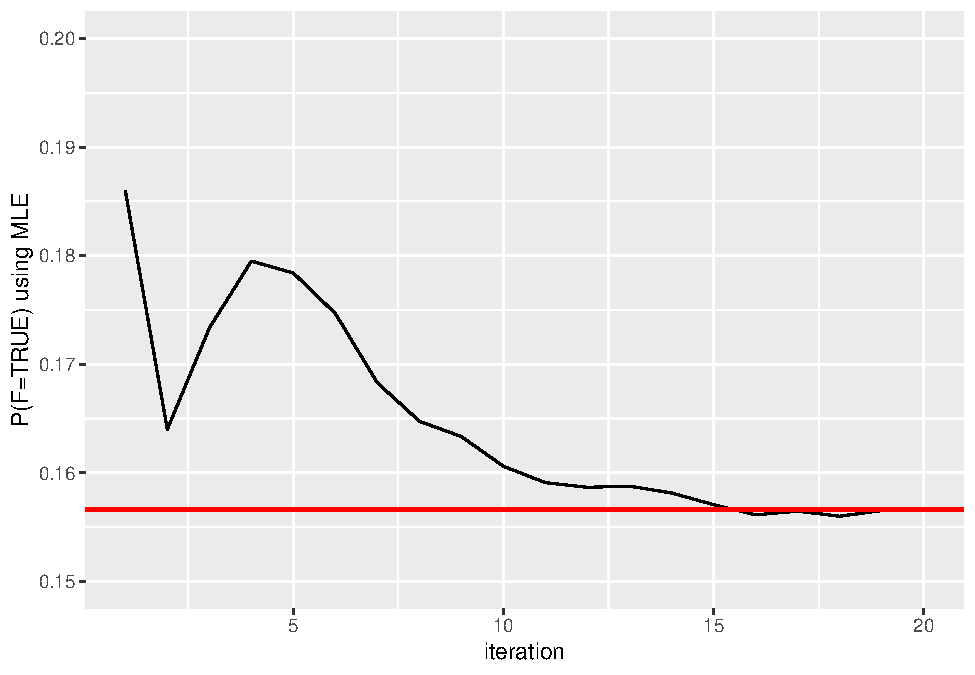
\includegraphics{bayesian_networks_files/figure-latex/unnamed-chunk-5-1.pdf}

Plotting P(F=TRUE) using bayes:

\begin{Shaded}
\begin{Highlighting}[]
\NormalTok{first.bayes }\CommentTok{\#Each iteration results}
\end{Highlighting}
\end{Shaded}

\begin{verbatim}
##  [1] 0.1921569 0.1673267 0.1754967 0.1810945 0.1796813 0.1757475 0.1692308
##  [8] 0.1655860 0.1640798 0.1612774 0.1597096 0.1592346 0.1592934 0.1586305
## [15] 0.1575233 0.1565543 0.1568743 0.1563818 0.1568875 0.1569431
\end{verbatim}

\begin{Shaded}
\begin{Highlighting}[]
\NormalTok{first.bayes }\OtherTok{\textless{}{-}} \FunctionTok{as.data.frame}\NormalTok{(first.bayes)}
\NormalTok{first.bayes}\SpecialCharTok{$}\NormalTok{ssize }\OtherTok{\textless{}{-}} \DecValTok{1}\SpecialCharTok{:}\DecValTok{20} \CommentTok{\# add iteration column}
\FunctionTok{ggplot}\NormalTok{(first.bayes, }\FunctionTok{aes}\NormalTok{(ssize, first.bayes)) }\SpecialCharTok{+} \FunctionTok{geom\_line}\NormalTok{() }\SpecialCharTok{+} \FunctionTok{geom\_hline}\NormalTok{(}\AttributeTok{yintercept =} \FloatTok{0.1569431}\NormalTok{, }\AttributeTok{color=}\StringTok{"red"}\NormalTok{, }\AttributeTok{size=}\DecValTok{1}\NormalTok{) }\SpecialCharTok{+} \FunctionTok{xlab}\NormalTok{(}\StringTok{"iteration"}\NormalTok{) }\SpecialCharTok{+} \FunctionTok{ylab}\NormalTok{(}\StringTok{"P(F=TRUE) using BAYES"}\NormalTok{) }\SpecialCharTok{+} \FunctionTok{ylim}\NormalTok{(}\FunctionTok{range}\NormalTok{(}\FloatTok{0.15}\NormalTok{,}\FloatTok{0.2}\NormalTok{))}
\end{Highlighting}
\end{Shaded}

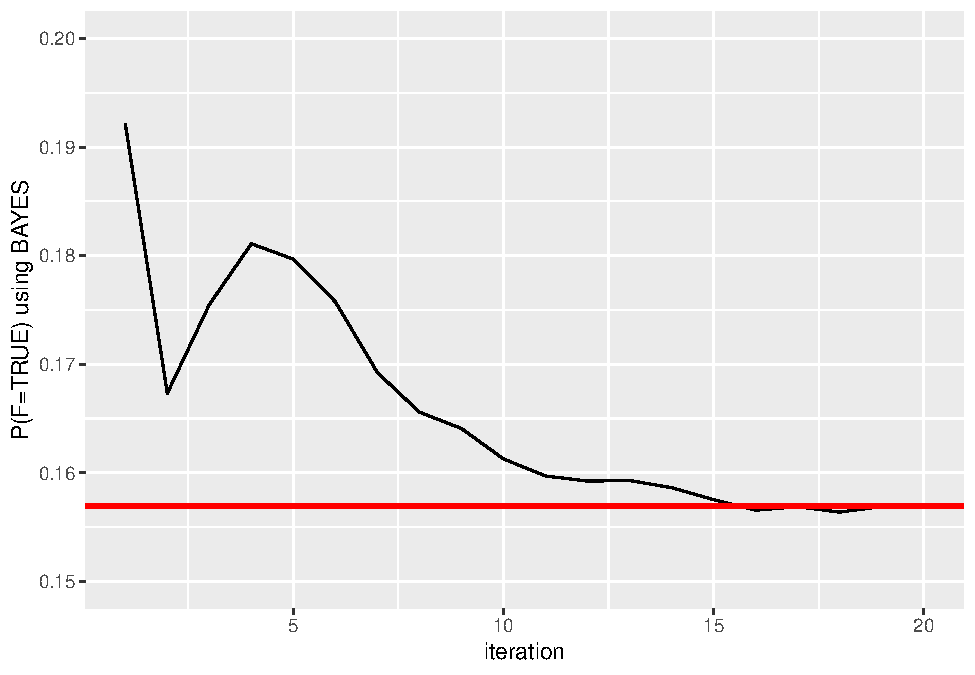
\includegraphics{bayesian_networks_files/figure-latex/unnamed-chunk-6-1.pdf}

Plotting P(F=TRUE) comparing both mle and bayes methods:

\begin{Shaded}
\begin{Highlighting}[]
\FunctionTok{plot}\NormalTok{(first.mle[,}\DecValTok{1}\NormalTok{], }\AttributeTok{type=}\StringTok{"l"}\NormalTok{, }\AttributeTok{col=}\StringTok{"red"}\NormalTok{, }\AttributeTok{lwd =} \DecValTok{2}\NormalTok{, }\AttributeTok{xlab=}\StringTok{"iteration"}\NormalTok{, }\AttributeTok{ylab=}\StringTok{"P(F=TRUE)"}\NormalTok{, }\AttributeTok{ylim=}\FunctionTok{range}\NormalTok{(}\FloatTok{0.15}\NormalTok{,}\FloatTok{0.20}\NormalTok{), }\AttributeTok{main=}\StringTok{"Plotting both methods"}\NormalTok{)}
\FunctionTok{lines}\NormalTok{(first.bayes[,}\DecValTok{1}\NormalTok{], }\AttributeTok{type=}\StringTok{"l"}\NormalTok{, }\AttributeTok{col=}\StringTok{"green"}\NormalTok{, }\AttributeTok{lwd =} \DecValTok{2}\NormalTok{)}
\FunctionTok{legend}\NormalTok{(}\StringTok{"topright"}\NormalTok{, }\AttributeTok{legend =} \FunctionTok{c}\NormalTok{(}\StringTok{"MLE"}\NormalTok{, }\StringTok{"BAYES"}\NormalTok{), }\AttributeTok{col =} \FunctionTok{c}\NormalTok{(}\StringTok{"red"}\NormalTok{,}\StringTok{"green"}\NormalTok{), }\AttributeTok{bty=}\StringTok{\textquotesingle{}n\textquotesingle{}}\NormalTok{, }\AttributeTok{lty=}\DecValTok{1}\NormalTok{, }\AttributeTok{lwd=}\DecValTok{2}\NormalTok{)}
\end{Highlighting}
\end{Shaded}

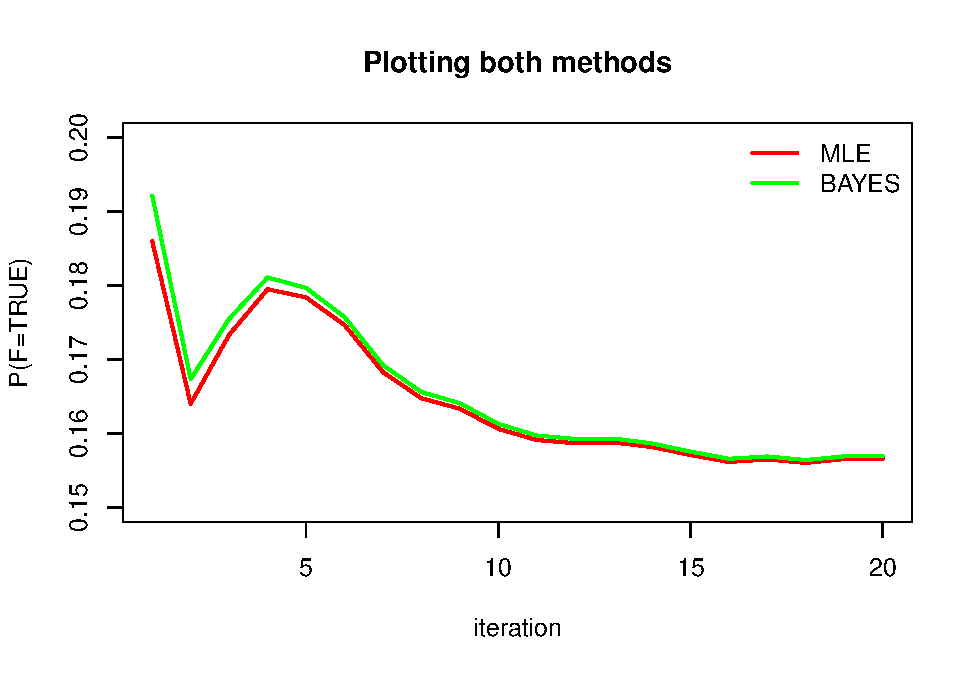
\includegraphics{bayesian_networks_files/figure-latex/unnamed-chunk-7-1.pdf}

Plotting P(D=OUT \textbar{} B=YES, F=TRUE) using mle:

\begin{Shaded}
\begin{Highlighting}[]
\NormalTok{second.mle }\CommentTok{\#Each iteration results}
\end{Highlighting}
\end{Shaded}

\begin{verbatim}
##  [1] 1 1 1 1 1 1 1 1 1 1 1 1 1 1 1 1 1 1 1 1
\end{verbatim}

\begin{Shaded}
\begin{Highlighting}[]
\NormalTok{second.mle }\OtherTok{\textless{}{-}} \FunctionTok{as.data.frame}\NormalTok{(second.mle)}
\NormalTok{second.mle}\SpecialCharTok{$}\NormalTok{ssize }\OtherTok{\textless{}{-}} \DecValTok{1}\SpecialCharTok{:}\DecValTok{20} \CommentTok{\# add iteration column}
\FunctionTok{ggplot}\NormalTok{(second.mle, }\FunctionTok{aes}\NormalTok{(ssize, second.mle)) }\SpecialCharTok{+} \FunctionTok{geom\_line}\NormalTok{() }\SpecialCharTok{+} \FunctionTok{geom\_hline}\NormalTok{(}\AttributeTok{yintercept =} \DecValTok{1}\NormalTok{, }\AttributeTok{color=}\StringTok{"red"}\NormalTok{, }\AttributeTok{size=}\DecValTok{1}\NormalTok{) }\SpecialCharTok{+} \FunctionTok{xlab}\NormalTok{(}\StringTok{"iteration"}\NormalTok{) }\SpecialCharTok{+} \FunctionTok{ylab}\NormalTok{(}\StringTok{"P(D=OUT | B=YES, F=TRUE) using MLE"}\NormalTok{) }\SpecialCharTok{+} \FunctionTok{ylim}\NormalTok{(}\FunctionTok{range}\NormalTok{(}\DecValTok{0}\NormalTok{,}\DecValTok{1}\NormalTok{))}
\end{Highlighting}
\end{Shaded}

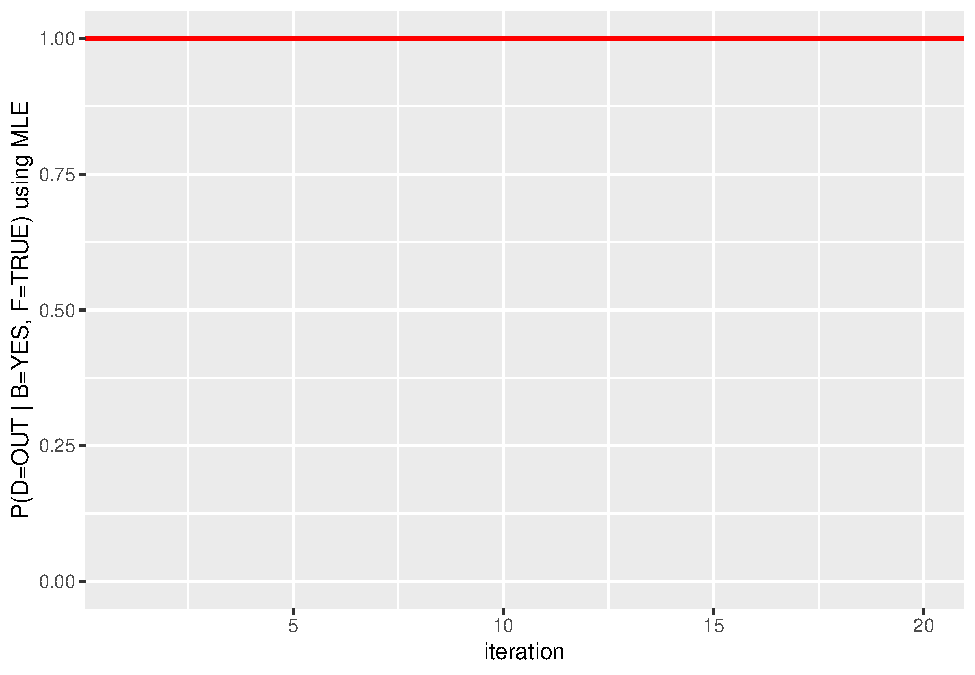
\includegraphics{bayesian_networks_files/figure-latex/unnamed-chunk-8-1.pdf}

Plotting P(D=OUT \textbar{} B=YES, F=TRUE) using bayes:

\begin{Shaded}
\begin{Highlighting}[]
\NormalTok{second.bayes }\CommentTok{\#Each iteration results}
\end{Highlighting}
\end{Shaded}

\begin{verbatim}
##  [1] 0.6428571 0.6428571 0.6428571 0.7222222 0.7727273 0.7727273 0.7727273
##  [8] 0.8076923 0.8333333 0.8529412 0.8529412 0.8809524 0.8809524 0.9000000
## [15] 0.9000000 0.9074074 0.9193548 0.9242424 0.9324324 0.9324324
\end{verbatim}

\begin{Shaded}
\begin{Highlighting}[]
\NormalTok{second.bayes }\OtherTok{\textless{}{-}} \FunctionTok{as.data.frame}\NormalTok{(second.bayes)}
\NormalTok{second.bayes}\SpecialCharTok{$}\NormalTok{ssize }\OtherTok{\textless{}{-}} \DecValTok{1}\SpecialCharTok{:}\DecValTok{20} \CommentTok{\# add iteration column}
\FunctionTok{ggplot}\NormalTok{(second.bayes, }\FunctionTok{aes}\NormalTok{(ssize, second.bayes)) }\SpecialCharTok{+} \FunctionTok{geom\_line}\NormalTok{() }\SpecialCharTok{+} \FunctionTok{geom\_hline}\NormalTok{(}\AttributeTok{yintercept =} \FloatTok{0.9324324}\NormalTok{, }\AttributeTok{color=}\StringTok{"red"}\NormalTok{, }\AttributeTok{size=}\DecValTok{1}\NormalTok{) }\SpecialCharTok{+} \FunctionTok{xlab}\NormalTok{(}\StringTok{"iteration"}\NormalTok{) }\SpecialCharTok{+} \FunctionTok{ylab}\NormalTok{(}\StringTok{"P(D=OUT | B=YES, F=TRUE) using BAYES"}\NormalTok{) }\SpecialCharTok{+} \FunctionTok{ylim}\NormalTok{(}\FunctionTok{range}\NormalTok{(}\DecValTok{0}\NormalTok{,}\DecValTok{1}\NormalTok{))}
\end{Highlighting}
\end{Shaded}

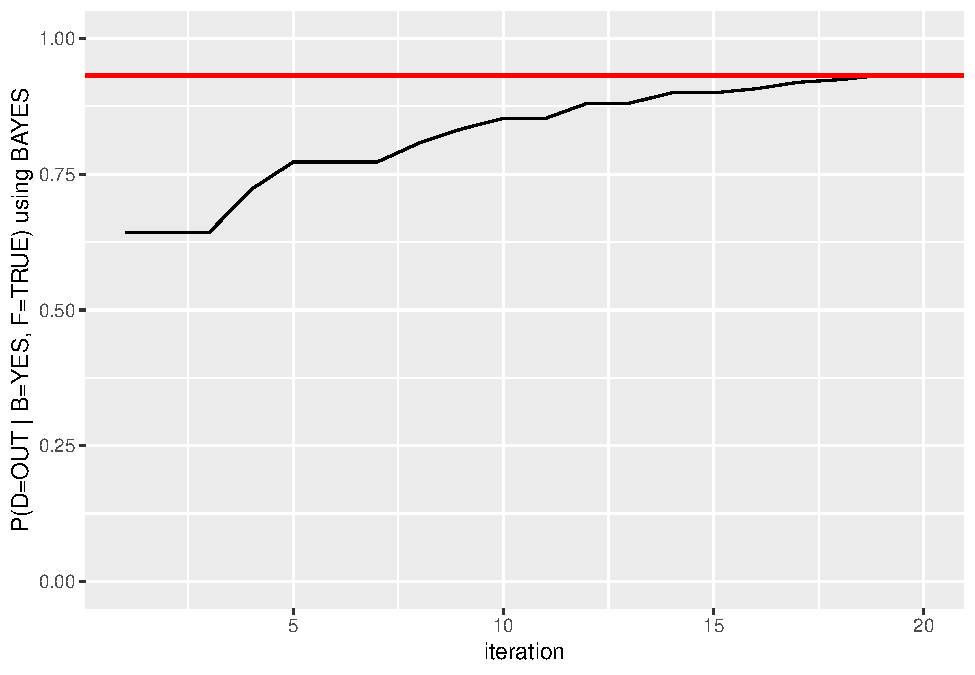
\includegraphics{bayesian_networks_files/figure-latex/unnamed-chunk-9-1.pdf}

Plotting P(D=OUT \textbar{} B=YES, F=TRUE) comparing both mle and bayes methods:

\begin{Shaded}
\begin{Highlighting}[]
\FunctionTok{plot}\NormalTok{(second.mle[,}\DecValTok{1}\NormalTok{], }\AttributeTok{type=}\StringTok{"l"}\NormalTok{, }\AttributeTok{col=}\StringTok{"red"}\NormalTok{, }\AttributeTok{lwd =} \DecValTok{2}\NormalTok{, }\AttributeTok{xlab=}\StringTok{"iteration"}\NormalTok{, }\AttributeTok{ylab=}\StringTok{"P(D=OUT | B=YES, F=TRUE)"}\NormalTok{, }\AttributeTok{ylim=}\FunctionTok{range}\NormalTok{(}\FloatTok{0.6}\NormalTok{,}\DecValTok{1}\NormalTok{), }\AttributeTok{main=}\StringTok{"Plotting both methods"}\NormalTok{)}
\FunctionTok{lines}\NormalTok{(second.bayes[,}\DecValTok{1}\NormalTok{], }\AttributeTok{type=}\StringTok{"l"}\NormalTok{, }\AttributeTok{col=}\StringTok{"green"}\NormalTok{, }\AttributeTok{lwd =} \DecValTok{2}\NormalTok{)}
\FunctionTok{legend}\NormalTok{(}\StringTok{"bottomright"}\NormalTok{, }\AttributeTok{legend =} \FunctionTok{c}\NormalTok{(}\StringTok{"MLE"}\NormalTok{, }\StringTok{"BAYES"}\NormalTok{), }\AttributeTok{col =} \FunctionTok{c}\NormalTok{(}\StringTok{"red"}\NormalTok{,}\StringTok{"green"}\NormalTok{), }\AttributeTok{bty=}\StringTok{\textquotesingle{}n\textquotesingle{}}\NormalTok{, }\AttributeTok{lty=}\DecValTok{1}\NormalTok{, }\AttributeTok{lwd=}\DecValTok{2}\NormalTok{)}
\end{Highlighting}
\end{Shaded}

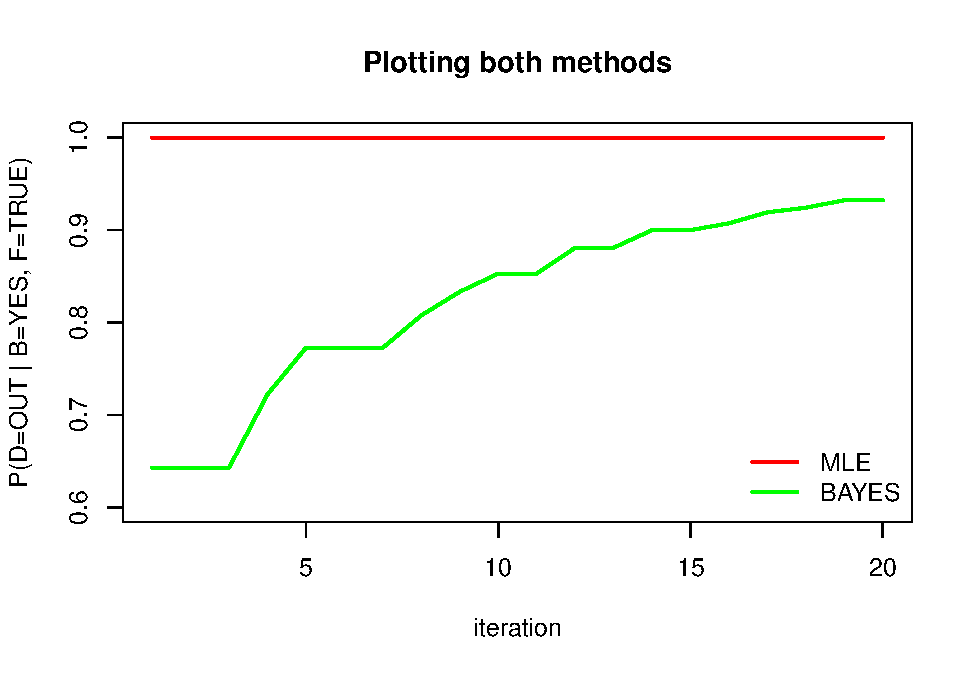
\includegraphics{bayesian_networks_files/figure-latex/unnamed-chunk-10-1.pdf}

\hypertarget{influence-diagrams}{%
\section{Influence Diagrams}\label{influence-diagrams}}

An influence diagram is:
- a directed acyclic graph G containing decision and chance nodes, and information and relevance arcs representing what is known at the time of a decision and probabilistic dependency, respectively.
- a set of probability distributions associated with each chance node,
- optionally a utility node and a corresponding set of utilities

\hypertarget{umbrella-problem}{%
\subsection{Umbrella Problem}\label{umbrella-problem}}

Consider the case when you are getting out of your apartment and you want to decide whether to take an umbrella with you or not. Your decision is certainly dependent on the weather, a phenomenon you cannot control. For simplicity, assume the weather can get one of the two states: sunshine or rain. You have likes and dislikes about taking your umbrella with you (you care!) depending on the weather. If it turns out to be a sunny day and you have taken your umbrella with you, you don't like it. However, you would hate it more if it rains and you do not have your umbrella. You are happier if it is sunny and you have left your umbrella at home (do not need to carry it around). You are happiest if it rains and you have your umbrella with you.

\begin{Shaded}
\begin{Highlighting}[]
\FunctionTok{library}\NormalTok{(HydeNet)}
\NormalTok{umbrella.net }\OtherTok{\textless{}{-}} \FunctionTok{HydeNetwork}\NormalTok{(}\SpecialCharTok{\textasciitilde{}}\NormalTok{ payoff }\SpecialCharTok{|}\NormalTok{ action}\SpecialCharTok{*}\NormalTok{weather)}
\end{Highlighting}
\end{Shaded}

For the chance node `weather':

\begin{Shaded}
\begin{Highlighting}[]
\NormalTok{weather\_prob }\OtherTok{\textless{}{-}} \FunctionTok{c}\NormalTok{(}\FloatTok{0.3}\NormalTok{, }\FloatTok{0.7}\NormalTok{) }\CommentTok{\#Prior probability for rain and sunshine, respectively.}
\NormalTok{umbrella.net }\OtherTok{\textless{}{-}} \FunctionTok{setNode}\NormalTok{(umbrella.net, weather, }\AttributeTok{nodeType=}\StringTok{"dcat"}\NormalTok{, }\AttributeTok{pi=}\FunctionTok{vectorProbs}\NormalTok{(}\AttributeTok{p=}\NormalTok{weather\_prob, weather), }\AttributeTok{factorLevels =} \FunctionTok{c}\NormalTok{(}\StringTok{"rain"}\NormalTok{,}\StringTok{"sunshine"}\NormalTok{), }\AttributeTok{validate =} \ConstantTok{FALSE}\NormalTok{)}
\end{Highlighting}
\end{Shaded}

For the decision nodes `action':

\begin{Shaded}
\begin{Highlighting}[]
\NormalTok{dprob }\OtherTok{\textless{}{-}} \FunctionTok{c}\NormalTok{(}\DecValTok{1}\NormalTok{,}\DecValTok{0}\NormalTok{) }\CommentTok{\#Probability of decision nodes represent do and don\textquotesingle{}t.}
\NormalTok{umbrella.net }\OtherTok{\textless{}{-}} \FunctionTok{setNode}\NormalTok{(umbrella.net, action, }\AttributeTok{nodeType=}\StringTok{"dcat"}\NormalTok{, }\AttributeTok{pi=}\FunctionTok{vectorProbs}\NormalTok{(}\AttributeTok{p=}\NormalTok{dprob, action), }\AttributeTok{factorLevels =} \FunctionTok{c}\NormalTok{(}\StringTok{"take"}\NormalTok{,}\StringTok{"leave"}\NormalTok{), }\AttributeTok{validate =} \ConstantTok{FALSE}\NormalTok{)}
\end{Highlighting}
\end{Shaded}

For the utility node `payoff':

\begin{Shaded}
\begin{Highlighting}[]
\NormalTok{umbrella.net }\OtherTok{\textless{}{-}} \FunctionTok{setNode}\NormalTok{(umbrella.net, payoff, }\StringTok{"determ"}\NormalTok{, }\AttributeTok{define=}\FunctionTok{fromFormula}\NormalTok{(),}
                  \AttributeTok{nodeFormula =}\NormalTok{ payoff }\SpecialCharTok{\textasciitilde{}} \FunctionTok{ifelse}\NormalTok{(weather }\SpecialCharTok{==} \StringTok{"rain"}\NormalTok{,}
                                                      \FunctionTok{ifelse}\NormalTok{(action }\SpecialCharTok{==} \StringTok{"take"}\NormalTok{, }\DecValTok{100}\NormalTok{, }\DecValTok{0}\NormalTok{),}
                                                             \FunctionTok{ifelse}\NormalTok{(action }\SpecialCharTok{==} \StringTok{"take"}\NormalTok{, }\DecValTok{30}\NormalTok{, }\DecValTok{70}\NormalTok{)))}

\NormalTok{umbrella.net }\OtherTok{\textless{}{-}} \FunctionTok{setDecisionNodes}\NormalTok{(umbrella.net, action) }\CommentTok{\#Setting the decision nodes}
\NormalTok{umbrella.net }\OtherTok{\textless{}{-}} \FunctionTok{setUtilityNodes}\NormalTok{(umbrella.net, payoff) }\CommentTok{\#Setting the utility nodes}
\FunctionTok{plot}\NormalTok{(umbrella.net) }\CommentTok{\#Plotting the influence diagram of extended version of oil{-}wildcatter problem}
\end{Highlighting}
\end{Shaded}


\includegraphics{bayesian_networks_files/figure-latex/unnamed-chunk-14-1.pdf}

\hypertarget{finding-the-optimal-policy}{%
\subsubsection{Finding the optimal policy}\label{finding-the-optimal-policy}}

Let us pass this structure to the Gibbs sampler (JAGS) and track the variables of interest (these nodes are useful to compute the conditional expectations if necessary).
Please note that the \texttt{rjags} package is just an interface to the JAGS library. Make sure you have installed JAGS-4.exe (can be downloaded from \href{http://www.sourceforge.net/projects/mcmc-jags/files}{here})
We are trying to compute the expected utility of the policy: (`action').
\texttt{HydeNet} provides a policyMatrix() function to enumerate all policies of a given decision network. This decision network is solved using Gibbs sampling with 10\^{}6 samples. We could use them as follows:

\begin{Shaded}
\begin{Highlighting}[]
\NormalTok{policy\_umbrella }\OtherTok{\textless{}{-}} \FunctionTok{policyMatrix}\NormalTok{(umbrella.net)}
\NormalTok{compiledNet\_umbrella }\OtherTok{\textless{}{-}} \FunctionTok{compileDecisionModel}\NormalTok{(umbrella.net, }\AttributeTok{policyMatrix =}\NormalTok{ policy\_umbrella)}
\end{Highlighting}
\end{Shaded}

\begin{verbatim}
## Compiling model graph
##    Resolving undeclared variables
##    Allocating nodes
## Graph information:
##    Observed stochastic nodes: 0
##    Unobserved stochastic nodes: 2
##    Total graph size: 16
## 
## Initializing model
## 
## Compiling model graph
##    Resolving undeclared variables
##    Allocating nodes
## Graph information:
##    Observed stochastic nodes: 1
##    Unobserved stochastic nodes: 1
##    Total graph size: 16
## 
## Initializing model
## 
## Compiling model graph
##    Resolving undeclared variables
##    Allocating nodes
## Graph information:
##    Observed stochastic nodes: 1
##    Unobserved stochastic nodes: 1
##    Total graph size: 16
## 
## Initializing model
\end{verbatim}

\begin{Shaded}
\begin{Highlighting}[]
\NormalTok{trackedVars\_umbrella }\OtherTok{\textless{}{-}} \FunctionTok{c}\NormalTok{(}\StringTok{"weather"}\NormalTok{,}\StringTok{"action"}\NormalTok{,}\StringTok{"payoff"}\NormalTok{)}
\NormalTok{samples\_umbrella }\OtherTok{\textless{}{-}} \FunctionTok{lapply}\NormalTok{(compiledNet\_umbrella,}
\NormalTok{                     HydeSim,}
                     \AttributeTok{variable.names =}\NormalTok{ trackedVars\_umbrella,}
                     \AttributeTok{n.iter =} \DecValTok{10}\SpecialCharTok{\^{}}\DecValTok{5}\NormalTok{)}
\end{Highlighting}
\end{Shaded}

Let us compute a single utility on samples:

\begin{Shaded}
\begin{Highlighting}[]
\NormalTok{samples\_umbrella }\OtherTok{\textless{}{-}} \FunctionTok{lapply}\NormalTok{(samples\_umbrella, }\ControlFlowTok{function}\NormalTok{(x) }
  \FunctionTok{cbind}\NormalTok{(x, }\AttributeTok{utility =}\NormalTok{ x}\SpecialCharTok{$}\NormalTok{payoff))}
\end{Highlighting}
\end{Shaded}

Now we can view all expectations at once by combining policies and the computed expectations:

\begin{Shaded}
\begin{Highlighting}[]
\NormalTok{results\_umbrella }\OtherTok{\textless{}{-}} \FunctionTok{lapply}\NormalTok{(samples\_umbrella, }\ControlFlowTok{function}\NormalTok{(l) }\FunctionTok{mean}\NormalTok{(l}\SpecialCharTok{$}\NormalTok{utility))}
\NormalTok{results\_umbrella }\OtherTok{\textless{}{-}} \FunctionTok{as.data.frame}\NormalTok{(}\FunctionTok{unlist}\NormalTok{(results\_umbrella))}
\NormalTok{results\_umbrella }\OtherTok{\textless{}{-}} \FunctionTok{cbind}\NormalTok{(policy\_umbrella, results\_umbrella)}
\FunctionTok{colnames}\NormalTok{(results\_umbrella)[}\FunctionTok{ncol}\NormalTok{(policy\_umbrella)}\SpecialCharTok{+}\DecValTok{1}\NormalTok{] }\OtherTok{\textless{}{-}} \StringTok{"utility"}
\end{Highlighting}
\end{Shaded}

The results according policies are given below:

\begin{Shaded}
\begin{Highlighting}[]
\NormalTok{results\_umbrella[]}
\end{Highlighting}
\end{Shaded}

\begin{verbatim}
##   action utility
## 1      1 50.9195
## 2      2 49.0588
\end{verbatim}

According to the policies, all utility values seem feasible and we don't have any conceptual error in the model.
The optimal policy seems to be:

\begin{Shaded}
\begin{Highlighting}[]
\NormalTok{results\_umbrella[results\_umbrella}\SpecialCharTok{$}\NormalTok{utility }\SpecialCharTok{==} \FunctionTok{max}\NormalTok{(results\_umbrella}\SpecialCharTok{$}\NormalTok{utility),] }
\end{Highlighting}
\end{Shaded}

\begin{verbatim}
##   action utility
## 1      1 50.9195
\end{verbatim}

..the first policy which means DO the `action', or TAKE the UMBRELLA which results in an expected reward of app. 51.2\%.

As extra information to be obtained from the output (to double check the validity of this model in this case),

Among the cases where it is decided not to ?drill? (3,4,7 and 8), it is sensible that the decision of not doing ?test? and not doing ?recovery? must be taken. It is clearly seen from result table.
So when you do drill, you simply do not ?test?. The utility results can be seen from the following table:

\begin{Shaded}
\begin{Highlighting}[]
\FunctionTok{lapply}\NormalTok{(samples\_umbrella, }\ControlFlowTok{function}\NormalTok{(l) }\FunctionTok{mean}\NormalTok{(l[l}\SpecialCharTok{$}\NormalTok{weather}\SpecialCharTok{==}\StringTok{"rain"}\NormalTok{,]}\SpecialCharTok{$}\NormalTok{utility))}
\end{Highlighting}
\end{Shaded}

\begin{verbatim}
## [[1]]
## [1] 100
## 
## [[2]]
## [1] 0
\end{verbatim}

\begin{Shaded}
\begin{Highlighting}[]
\FunctionTok{lapply}\NormalTok{(samples\_umbrella, }\ControlFlowTok{function}\NormalTok{(l) }\FunctionTok{mean}\NormalTok{(l[l}\SpecialCharTok{$}\NormalTok{weather}\SpecialCharTok{==}\StringTok{"sunshine"}\NormalTok{,]}\SpecialCharTok{$}\NormalTok{utility))}
\end{Highlighting}
\end{Shaded}

\begin{verbatim}
## [[1]]
## [1] 30
## 
## [[2]]
## [1] 70
\end{verbatim}

\hypertarget{evaluating-influence-diagrams-augmented-variable-elimination}{%
\paragraph{Evaluating Influence Diagrams: Augmented Variable Elimination}\label{evaluating-influence-diagrams-augmented-variable-elimination}}

\begin{itemize}
\tightlist
\item
  \emph{Barren node removal}: A barren node may be simply removed from an oriented, regular influence diagram. If it is a decision node, then any alternative would be optimal.
\item
  \emph{Chance node removal}: Given that chance node X directly precedes the value node and nothing else in an oriented, regular ID, node X can be removed by conditional expectation. Afterward, the value node inherits all of the conditional predecessors from node X, and thus the process creates no new barren nodes.
\item
  \emph{Decision node removal}: Given that all barren nodes have been removed, that decision node A is a conditional predecessor of the value node, and that all other conditional predecessors of the value node are informational predecessors of node A in an oriented, regular ID, node A may be removed by maximizing expected utility, conditioned on the values of its informational predecessors. The maximizing alternative(s) should be recorded as the optimal policy.
\item
  \emph{Arc reversal}: (between chance nodes). As we have seen before.
\end{itemize}

\hypertarget{incorporating-weather-forecast}{%
\subsection{Incorporating Weather Forecast}\label{incorporating-weather-forecast}}

Consider the umbrella problem. Assume that you now decided to make a more \textbf{informed} decision. You listen to a weather forecast for that day. The new situation is depicted as:

\begin{Shaded}
\begin{Highlighting}[]
\FunctionTok{library}\NormalTok{(HydeNet)}
\NormalTok{umbrella2.net }\OtherTok{\textless{}{-}} \FunctionTok{HydeNetwork}\NormalTok{(}\SpecialCharTok{\textasciitilde{}}\NormalTok{ payoff }\SpecialCharTok{|}\NormalTok{ action}\SpecialCharTok{*}\NormalTok{weather}
                             \SpecialCharTok{+}\NormalTok{ action }\SpecialCharTok{|}\NormalTok{ weather\_forecast}
                             \SpecialCharTok{+}\NormalTok{ weather\_forecast }\SpecialCharTok{|}\NormalTok{ weather)}
\end{Highlighting}
\end{Shaded}

For the chance node `weather':

\begin{Shaded}
\begin{Highlighting}[]
\NormalTok{weather\_prob }\OtherTok{\textless{}{-}} \FunctionTok{c}\NormalTok{(}\FloatTok{0.3}\NormalTok{,}\FloatTok{0.7}\NormalTok{) }\CommentTok{\#Prior probability for rain and sunshine, respectively.}
\NormalTok{umbrella2.net }\OtherTok{\textless{}{-}} \FunctionTok{setNode}\NormalTok{(umbrella2.net, weather, }\AttributeTok{nodeType=}\StringTok{"dcat"}\NormalTok{, }\AttributeTok{pi=}\FunctionTok{vectorProbs}\NormalTok{(}\AttributeTok{p=}\NormalTok{weather\_prob, weather), }\AttributeTok{factorLevels =} \FunctionTok{c}\NormalTok{(}\StringTok{"rain"}\NormalTok{,}\StringTok{"sunshine"}\NormalTok{), }\AttributeTok{validate =} \ConstantTok{FALSE}\NormalTok{)}
\end{Highlighting}
\end{Shaded}

For the chance node `weather\_forecast':

\begin{Shaded}
\begin{Highlighting}[]
\NormalTok{cpt\_weather\_forecast }\OtherTok{\textless{}{-}} \FunctionTok{readRDS}\NormalTok{(}\FunctionTok{url}\NormalTok{(}\StringTok{"https://github.com/canaytore/bayesian{-}networks/raw/main/data/cpt\_weather\_forecast.rds"}\NormalTok{))}
\CommentTok{\#The file ?cpt\_weather\_forecast.rds? was created using the inputCPT() function of HydeNet. It stands for the conditional probability table of the seismic results based on parent nodes which are \textquotesingle{}test\textquotesingle{} and \textquotesingle{}oil\_content\textquotesingle{}.}
\NormalTok{cpt\_weather\_forecast}
\end{Highlighting}
\end{Shaded}

\begin{verbatim}
##           weather_forecast
## weather    sunny cloudy rainy
##   rain      0.15   0.25   0.6
##   sunshine  0.70   0.20   0.1
\end{verbatim}

\begin{Shaded}
\begin{Highlighting}[]
\NormalTok{umbrella2.net }\OtherTok{\textless{}{-}} \FunctionTok{setNodeModels}\NormalTok{(umbrella2.net, cpt\_weather\_forecast)}
\end{Highlighting}
\end{Shaded}

For the decision nodes `action':

\begin{Shaded}
\begin{Highlighting}[]
\NormalTok{dprob }\OtherTok{\textless{}{-}} \FunctionTok{c}\NormalTok{(}\DecValTok{1}\NormalTok{,}\DecValTok{0}\NormalTok{) }\CommentTok{\#Probability of decision nodes represent do and don\textquotesingle{}t.}
\NormalTok{umbrella2.net }\OtherTok{\textless{}{-}} \FunctionTok{setNode}\NormalTok{(umbrella2.net, action, }\AttributeTok{nodeType=}\StringTok{"dcat"}\NormalTok{, }\AttributeTok{pi=}\FunctionTok{vectorProbs}\NormalTok{(}\AttributeTok{p=}\NormalTok{dprob, action), }\AttributeTok{factorLevels =} \FunctionTok{c}\NormalTok{(}\StringTok{"take"}\NormalTok{,}\StringTok{"leave"}\NormalTok{), }\AttributeTok{validate =} \ConstantTok{FALSE}\NormalTok{)}
\end{Highlighting}
\end{Shaded}

For the utility node `payoff':

\begin{Shaded}
\begin{Highlighting}[]
\NormalTok{umbrella2.net }\OtherTok{\textless{}{-}} \FunctionTok{setNode}\NormalTok{(umbrella2.net, payoff, }\StringTok{"determ"}\NormalTok{, }\AttributeTok{define=}\FunctionTok{fromFormula}\NormalTok{(),}
                  \AttributeTok{nodeFormula =}\NormalTok{ payoff }\SpecialCharTok{\textasciitilde{}} \FunctionTok{ifelse}\NormalTok{(weather }\SpecialCharTok{==} \StringTok{"rain"}\NormalTok{,}
                                                      \FunctionTok{ifelse}\NormalTok{(action }\SpecialCharTok{==} \StringTok{"take"}\NormalTok{, }\DecValTok{100}\NormalTok{, }\DecValTok{0}\NormalTok{),}
                                                             \FunctionTok{ifelse}\NormalTok{(action }\SpecialCharTok{==} \StringTok{"take"}\NormalTok{, }\DecValTok{30}\NormalTok{, }\DecValTok{70}\NormalTok{)))}

\NormalTok{umbrella2.net }\OtherTok{\textless{}{-}} \FunctionTok{setDecisionNodes}\NormalTok{(umbrella2.net, action) }\CommentTok{\#Setting the decision nodes}
\NormalTok{umbrella2.net }\OtherTok{\textless{}{-}} \FunctionTok{setUtilityNodes}\NormalTok{(umbrella2.net, payoff) }\CommentTok{\#Setting the utility nodes}
\FunctionTok{plot}\NormalTok{(umbrella2.net) }\CommentTok{\#Plotting the influence diagram of extended version of oil{-}wildcatter problem}
\end{Highlighting}
\end{Shaded}


\includegraphics{bayesian_networks_files/figure-latex/unnamed-chunk-25-1.pdf}

\hypertarget{finding-the-optimal-policy-1}{%
\subsubsection{Finding the optimal policy}\label{finding-the-optimal-policy-1}}

Let us pass this structure to the Gibbs sampler (JAGS) and track the variables of interest (these nodes are useful to compute the conditional expectations if necessary).
Please note that the \texttt{rjags} package is just an interface to the JAGS library. Make sure you have installed JAGS-4.exe (can be downloaded from \href{http://www.sourceforge.net/projects/mcmc-jags/files}{here})
We are trying to compute the expected utility of the policy: (`action').
\texttt{HydeNet} provides a policyMatrix() function to enumerate all policies of a given decision network. This decision network is solved using Gibbs sampling with 10\^{}6 samples. We could use them as follows:

\begin{Shaded}
\begin{Highlighting}[]
\NormalTok{policy\_umbrella2 }\OtherTok{\textless{}{-}} \FunctionTok{policyMatrix}\NormalTok{(umbrella2.net)}
\NormalTok{compiledNet\_umbrella2 }\OtherTok{\textless{}{-}} \FunctionTok{compileDecisionModel}\NormalTok{(umbrella2.net, }\AttributeTok{policyMatrix =}\NormalTok{ policy\_umbrella2)}
\end{Highlighting}
\end{Shaded}

\begin{verbatim}
## Compiling model graph
##    Resolving undeclared variables
##    Allocating nodes
## Graph information:
##    Observed stochastic nodes: 0
##    Unobserved stochastic nodes: 3
##    Total graph size: 26
## 
## Initializing model
## 
## Compiling model graph
##    Resolving undeclared variables
##    Allocating nodes
## Graph information:
##    Observed stochastic nodes: 1
##    Unobserved stochastic nodes: 2
##    Total graph size: 26
## 
## Initializing model
## 
## Compiling model graph
##    Resolving undeclared variables
##    Allocating nodes
## Graph information:
##    Observed stochastic nodes: 1
##    Unobserved stochastic nodes: 2
##    Total graph size: 26
## 
## Initializing model
\end{verbatim}

\begin{Shaded}
\begin{Highlighting}[]
\NormalTok{trackedVars\_umbrella2 }\OtherTok{\textless{}{-}} \FunctionTok{c}\NormalTok{(}\StringTok{"weather"}\NormalTok{,}\StringTok{"weather\_forecast"}\NormalTok{,}\StringTok{"action"}\NormalTok{,}\StringTok{"payoff"}\NormalTok{)}
\NormalTok{samples\_umbrella2 }\OtherTok{\textless{}{-}} \FunctionTok{lapply}\NormalTok{(compiledNet\_umbrella2,}
\NormalTok{                     HydeSim,}
                     \AttributeTok{variable.names =}\NormalTok{ trackedVars\_umbrella2,}
                     \AttributeTok{n.iter =} \DecValTok{10}\SpecialCharTok{\^{}}\DecValTok{5}\NormalTok{)}
\end{Highlighting}
\end{Shaded}

Let us compute a single utility on samples:

\begin{Shaded}
\begin{Highlighting}[]
\NormalTok{samples\_umbrella2 }\OtherTok{\textless{}{-}} \FunctionTok{lapply}\NormalTok{(samples\_umbrella2, }\ControlFlowTok{function}\NormalTok{(x) }
  \FunctionTok{cbind}\NormalTok{(x, }\AttributeTok{utility =}\NormalTok{ x}\SpecialCharTok{$}\NormalTok{payoff))}
\end{Highlighting}
\end{Shaded}

Now we can view all expectations at once by combining policies and the computed expectations:

\begin{Shaded}
\begin{Highlighting}[]
\NormalTok{results\_umbrella2 }\OtherTok{\textless{}{-}} \FunctionTok{lapply}\NormalTok{(samples\_umbrella2, }\ControlFlowTok{function}\NormalTok{(l) }\FunctionTok{mean}\NormalTok{(l}\SpecialCharTok{$}\NormalTok{utility))}
\NormalTok{results\_umbrella2 }\OtherTok{\textless{}{-}} \FunctionTok{as.data.frame}\NormalTok{(}\FunctionTok{unlist}\NormalTok{(results\_umbrella2))}
\NormalTok{results\_umbrella2 }\OtherTok{\textless{}{-}} \FunctionTok{cbind}\NormalTok{(policy\_umbrella2, results\_umbrella2)}
\FunctionTok{colnames}\NormalTok{(results\_umbrella2)[}\FunctionTok{ncol}\NormalTok{(policy\_umbrella2)}\SpecialCharTok{+}\DecValTok{1}\NormalTok{] }\OtherTok{\textless{}{-}} \StringTok{"utility"}
\end{Highlighting}
\end{Shaded}

The results according policies are given below:

\begin{Shaded}
\begin{Highlighting}[]
\NormalTok{results\_umbrella2[]}
\end{Highlighting}
\end{Shaded}

\begin{verbatim}
##   action utility
## 1      1 51.0049
## 2      2 49.0035
\end{verbatim}

According to the policies, all utility values seem feasible and we don't have any conceptual error in the model.
The optimal policy seems to be:

\begin{Shaded}
\begin{Highlighting}[]
\NormalTok{results\_umbrella2[results\_umbrella2}\SpecialCharTok{$}\NormalTok{utility }\SpecialCharTok{==} \FunctionTok{max}\NormalTok{(results\_umbrella2}\SpecialCharTok{$}\NormalTok{utility),] }
\end{Highlighting}
\end{Shaded}

\begin{verbatim}
##   action utility
## 1      1 51.0049
\end{verbatim}

..the first policy which means DO the `action', or TAKE the UMBRELLA which results in an expected reward of app. 51.2\%.

As extra information to be obtained from the output (also to double check the validity of this model in this case),

Among the cases where it is decided not to ?drill? (3,4,7 and 8), it is sensible that the decision of not doing ?test? and not doing ?recovery? must be taken. It is clearly seen from result table.
So when you do drill, you simply do not ?test?. The utility results can be seen from the following table:

\begin{Shaded}
\begin{Highlighting}[]
\FunctionTok{lapply}\NormalTok{(samples\_umbrella2, }\ControlFlowTok{function}\NormalTok{(l) }\FunctionTok{mean}\NormalTok{(l[l}\SpecialCharTok{$}\NormalTok{weather\_forecast}\SpecialCharTok{==}\StringTok{"sunny"}\NormalTok{,]}\SpecialCharTok{$}\NormalTok{utility))}
\end{Highlighting}
\end{Shaded}

\begin{verbatim}
## [[1]]
## [1] 35.87268
## 
## [[2]]
## [1] 64.02429
\end{verbatim}

\begin{Shaded}
\begin{Highlighting}[]
\FunctionTok{lapply}\NormalTok{(samples\_umbrella2, }\ControlFlowTok{function}\NormalTok{(l) }\FunctionTok{mean}\NormalTok{(l[l}\SpecialCharTok{$}\NormalTok{weather\_forecast}\SpecialCharTok{==}\StringTok{"rainy"}\NormalTok{,]}\SpecialCharTok{$}\NormalTok{utility))}
\end{Highlighting}
\end{Shaded}

\begin{verbatim}
## [[1]]
## [1] 80.52193
## 
## [[2]]
## [1] 19.61979
\end{verbatim}

\begin{Shaded}
\begin{Highlighting}[]
\FunctionTok{lapply}\NormalTok{(samples\_umbrella2, }\ControlFlowTok{function}\NormalTok{(l) }\FunctionTok{mean}\NormalTok{(l[l}\SpecialCharTok{$}\NormalTok{weather\_forecast}\SpecialCharTok{==}\StringTok{"cloudy"}\NormalTok{,]}\SpecialCharTok{$}\NormalTok{utility))}
\end{Highlighting}
\end{Shaded}

\begin{verbatim}
## [[1]]
## [1] 54.25092
## 
## [[2]]
## [1] 45.69221
\end{verbatim}

\hypertarget{oil-wildcatter-problem}{%
\subsection{Oil-Wildcatter Problem:}\label{oil-wildcatter-problem}}

An oil wildcatter must decide whether to drill or not to drill. The cost of drilling is \$70,000. If he decides to drill, the well may be soaking (with a return of \$270,000), wet (with a return of \$120,000), or dry (with a return of \$0). These returns are exclusive of the drilling cost. The prior probabilities for soaking (lots of oil), wet (some oil), and dry (no oil) are (0.2, 0.3, 0.5). At the cost of \$10,000, the oil wildcatter could decide to take seismic soundings of the geological structure at the site to classify the structure as having either no structure ns, open structure, os and closed structure cs. The specifics of the test are given as follows:

\begin{figure}
\centering
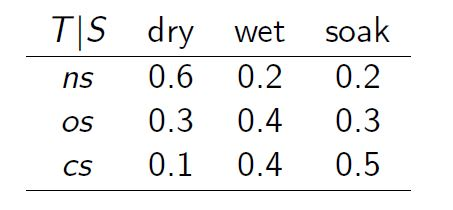
\includegraphics{data/cpt_test_soaking.JPG}
\caption{cpt\_test}
\end{figure}

\hypertarget{defining-the-extended-network-in-hydenet}{%
\subsubsection{Defining the extended network in HydeNet}\label{defining-the-extended-network-in-hydenet}}

Our first task will be to represent and solve the extended oil-wildcatter influence diagram using \texttt{HydeNet}. We generate the network in \texttt{HydeNet} as follows;

\begin{Shaded}
\begin{Highlighting}[]
\FunctionTok{library}\NormalTok{(HydeNet)}
\NormalTok{ow.net }\OtherTok{\textless{}{-}} \FunctionTok{HydeNetwork}\NormalTok{(}\SpecialCharTok{\textasciitilde{}}\NormalTok{ cost }\SpecialCharTok{|}\NormalTok{ test }
                      \SpecialCharTok{+}\NormalTok{ drill }\SpecialCharTok{|}\NormalTok{ test}\SpecialCharTok{*}\NormalTok{seismic\_results }
                      \SpecialCharTok{+}\NormalTok{ seismic\_results }\SpecialCharTok{|}\NormalTok{ test}\SpecialCharTok{*}\NormalTok{oil\_content }
                      \SpecialCharTok{+}\NormalTok{ reward }\SpecialCharTok{|}\NormalTok{ drill}\SpecialCharTok{*}\NormalTok{oil\_content)}
\end{Highlighting}
\end{Shaded}

For the chance node `oil\_content':

\begin{Shaded}
\begin{Highlighting}[]
\NormalTok{oil\_content\_prob }\OtherTok{\textless{}{-}} \FunctionTok{c}\NormalTok{(}\FloatTok{0.5}\NormalTok{, }\FloatTok{0.3}\NormalTok{, }\FloatTok{0.2}\NormalTok{) }\CommentTok{\#Prior probability for dry, wet and soaking, respectively.}
\NormalTok{ow.net }\OtherTok{\textless{}{-}} \FunctionTok{setNode}\NormalTok{(ow.net, oil\_content, }\AttributeTok{nodeType=}\StringTok{"dcat"}\NormalTok{, }\AttributeTok{pi=}\FunctionTok{vectorProbs}\NormalTok{(}\AttributeTok{p=}\NormalTok{oil\_content\_prob, oil\_content), }\AttributeTok{factorLevels =} \FunctionTok{c}\NormalTok{(}\StringTok{"dry"}\NormalTok{,}\StringTok{"wet"}\NormalTok{,}\StringTok{"soak"}\NormalTok{), }\AttributeTok{validate =} \ConstantTok{FALSE}\NormalTok{)}
\end{Highlighting}
\end{Shaded}

For the decision nodes `test' and `drill':

\begin{Shaded}
\begin{Highlighting}[]
\NormalTok{dprob }\OtherTok{\textless{}{-}} \FunctionTok{c}\NormalTok{(}\DecValTok{1}\NormalTok{,}\DecValTok{0}\NormalTok{) }\CommentTok{\#Probability of decision nodes represent do and don\textquotesingle{}t.}
\NormalTok{ow.net }\OtherTok{\textless{}{-}} \FunctionTok{setNode}\NormalTok{(ow.net, test, }\AttributeTok{nodeType=}\StringTok{"dcat"}\NormalTok{, }\AttributeTok{pi=}\FunctionTok{vectorProbs}\NormalTok{(}\AttributeTok{p=}\NormalTok{dprob, test), }\AttributeTok{factorLevels =} \FunctionTok{c}\NormalTok{(}\StringTok{"test"}\NormalTok{,}\StringTok{"dont\_test"}\NormalTok{), }\AttributeTok{validate =} \ConstantTok{FALSE}\NormalTok{)}
\NormalTok{ow.net }\OtherTok{\textless{}{-}} \FunctionTok{setNode}\NormalTok{(ow.net, drill, }\AttributeTok{nodeType=}\StringTok{"dcat"}\NormalTok{, }\AttributeTok{pi=}\FunctionTok{vectorProbs}\NormalTok{(}\AttributeTok{p=}\NormalTok{dprob, drill), }\AttributeTok{factorLevels =} \FunctionTok{c}\NormalTok{(}\StringTok{"drill"}\NormalTok{,}\StringTok{"dont\_drill"}\NormalTok{), }\AttributeTok{validate =} \ConstantTok{FALSE}\NormalTok{)}
\end{Highlighting}
\end{Shaded}

For the chance node `seismic\_results':

\begin{Shaded}
\begin{Highlighting}[]
\NormalTok{cpt\_seismic\_results }\OtherTok{\textless{}{-}} \FunctionTok{readRDS}\NormalTok{(}\FunctionTok{url}\NormalTok{(}\StringTok{"https://github.com/canaytore/bayesian{-}networks/raw/main/data/cpt\_seismic\_results.rds"}\NormalTok{))}
\CommentTok{\#The file ?cpt\_seismic\_results.rds? was created using the inputCPT() function of HydeNet. It stands for the conditional probability table of the seismic results based on parent nodes which are \textquotesingle{}test\textquotesingle{} and \textquotesingle{}oil\_content\textquotesingle{}.}
\NormalTok{cpt\_seismic\_results}
\end{Highlighting}
\end{Shaded}

\begin{verbatim}
## , , seismic_results = ns
## 
##            oil_content
## test         dry  wet soak
##   test      0.60 0.20 0.20
##   dont_test 0.33 0.33 0.33
## 
## , , seismic_results = os
## 
##            oil_content
## test         dry  wet soak
##   test      0.30 0.40 0.30
##   dont_test 0.33 0.33 0.33
## 
## , , seismic_results = cs
## 
##            oil_content
## test         dry  wet soak
##   test      0.10 0.40 0.50
##   dont_test 0.34 0.34 0.34
\end{verbatim}

\begin{Shaded}
\begin{Highlighting}[]
\NormalTok{ow.net }\OtherTok{\textless{}{-}} \FunctionTok{setNodeModels}\NormalTok{(ow.net, cpt\_seismic\_results)}
\end{Highlighting}
\end{Shaded}

For the utility node `cost':

\begin{Shaded}
\begin{Highlighting}[]
\NormalTok{ow.net }\OtherTok{\textless{}{-}} \FunctionTok{setNode}\NormalTok{(ow.net, cost, }\StringTok{"determ"}\NormalTok{, }\AttributeTok{define=}\FunctionTok{fromFormula}\NormalTok{(),}
                  \AttributeTok{nodeFormula =}\NormalTok{ cost }\SpecialCharTok{\textasciitilde{}} \FunctionTok{ifelse}\NormalTok{(test }\SpecialCharTok{==} \StringTok{"test"}\NormalTok{, }\SpecialCharTok{{-}}\DecValTok{10}\NormalTok{, }\DecValTok{0}\NormalTok{))}
\end{Highlighting}
\end{Shaded}

For the utility node `reward':

\begin{Shaded}
\begin{Highlighting}[]
\NormalTok{ow.net }\OtherTok{\textless{}{-}} \FunctionTok{setNode}\NormalTok{(ow.net, reward, }\StringTok{"determ"}\NormalTok{, }\AttributeTok{define=}\FunctionTok{fromFormula}\NormalTok{(),}
                  \AttributeTok{nodeFormula =}\NormalTok{ reward }\SpecialCharTok{\textasciitilde{}} \FunctionTok{ifelse}\NormalTok{(oil\_content }\SpecialCharTok{==} \StringTok{"dry"}\NormalTok{,}
                                                      \FunctionTok{ifelse}\NormalTok{(drill }\SpecialCharTok{==} \StringTok{"drill"}\NormalTok{, }\SpecialCharTok{{-}}\DecValTok{70}\NormalTok{, }\DecValTok{0}\NormalTok{),}
                                                      \FunctionTok{ifelse}\NormalTok{(oil\_content }\SpecialCharTok{==} \StringTok{"wet"}\NormalTok{,}
                                                             \FunctionTok{ifelse}\NormalTok{(drill }\SpecialCharTok{==} \StringTok{"drill"}\NormalTok{, }\DecValTok{50}\NormalTok{, }\DecValTok{0}\NormalTok{),}
                                                             \FunctionTok{ifelse}\NormalTok{(drill }\SpecialCharTok{==} \StringTok{"drill"}\NormalTok{, }\DecValTok{200}\NormalTok{, }\DecValTok{0}\NormalTok{))))}

\NormalTok{ow.net }\OtherTok{\textless{}{-}} \FunctionTok{setDecisionNodes}\NormalTok{(ow.net, test, drill) }\CommentTok{\#Setting the decision nodes}
\NormalTok{ow.net }\OtherTok{\textless{}{-}} \FunctionTok{setUtilityNodes}\NormalTok{(ow.net, cost, reward) }\CommentTok{\#Setting the utility nodes}
\FunctionTok{plot}\NormalTok{(ow.net) }\CommentTok{\#Plotting the influence diagram of extended version of oil{-}wildcatter problem}
\end{Highlighting}
\end{Shaded}


\includegraphics{bayesian_networks_files/figure-latex/unnamed-chunk-37-1.pdf}

The trick is here that we will have precise information about `oil\_content' after the decision `drill'.
Besides, there must be an arc from ?drill? to ?recovery\_level? since `recovery\_level' should exactly be nr (no recovery) when the drill is not done since it is not sensible to be able to do secondary `recovery' without the primary `drill'.

\hypertarget{finding-the-optimal-policy-2}{%
\subsubsection{Finding the optimal policy}\label{finding-the-optimal-policy-2}}

Let us pass this structure to the Gibbs sampler (JAGS) and track the variables of interest (these nodes are useful to compute the conditional expectations if necessary).
Please note that the \texttt{rjags} package is just an interface to the JAGS library. Make sure you have installed JAGS-4.exe (can be downloaded from \href{http://www.sourceforge.net/projects/mcmc-jags/files}{here})
We are trying to compute the expected utility of the policy: (`action').
\texttt{HydeNet} provides a policyMatrix() function to enumerate all policies of a given decision network. This decision network is solved using Gibbs sampling with 10\^{}6 samples. We could use them as follows:

\begin{Shaded}
\begin{Highlighting}[]
\NormalTok{policy\_ow }\OtherTok{\textless{}{-}} \FunctionTok{policyMatrix}\NormalTok{(ow.net)}
\NormalTok{compiledNet\_ow }\OtherTok{\textless{}{-}} \FunctionTok{compileDecisionModel}\NormalTok{(ow.net, }\AttributeTok{policyMatrix =}\NormalTok{ policy\_ow)}
\end{Highlighting}
\end{Shaded}

\begin{verbatim}
## Compiling model graph
##    Resolving undeclared variables
##    Allocating nodes
## Graph information:
##    Observed stochastic nodes: 0
##    Unobserved stochastic nodes: 4
##    Total graph size: 54
## 
## Initializing model
## 
## Compiling model graph
##    Resolving undeclared variables
##    Allocating nodes
## Graph information:
##    Observed stochastic nodes: 2
##    Unobserved stochastic nodes: 2
##    Total graph size: 50
## 
## Initializing model
## 
## Compiling model graph
##    Resolving undeclared variables
##    Allocating nodes
## Graph information:
##    Observed stochastic nodes: 2
##    Unobserved stochastic nodes: 2
##    Total graph size: 51
## 
## Initializing model
## 
## Compiling model graph
##    Resolving undeclared variables
##    Allocating nodes
## Graph information:
##    Observed stochastic nodes: 2
##    Unobserved stochastic nodes: 2
##    Total graph size: 51
## 
## Initializing model
## 
## Compiling model graph
##    Resolving undeclared variables
##    Allocating nodes
## Graph information:
##    Observed stochastic nodes: 2
##    Unobserved stochastic nodes: 2
##    Total graph size: 50
## 
## Initializing model
\end{verbatim}

\begin{Shaded}
\begin{Highlighting}[]
\NormalTok{trackedVars\_ow }\OtherTok{\textless{}{-}} \FunctionTok{c}\NormalTok{(}\StringTok{"oil\_content"}\NormalTok{,}\StringTok{"seismic\_results"}\NormalTok{,}\StringTok{"test"}\NormalTok{,}\StringTok{"cost"}\NormalTok{,}\StringTok{"drill"}\NormalTok{,}\StringTok{"reward"}\NormalTok{)}
\NormalTok{samples\_ow }\OtherTok{\textless{}{-}} \FunctionTok{lapply}\NormalTok{(compiledNet\_ow,}
\NormalTok{                     HydeSim,}
                     \AttributeTok{variable.names =}\NormalTok{ trackedVars\_ow,}
                     \AttributeTok{n.iter =} \DecValTok{10}\SpecialCharTok{\^{}}\DecValTok{5}\NormalTok{)}
\end{Highlighting}
\end{Shaded}

Let us compute a single utility on samples:

\begin{Shaded}
\begin{Highlighting}[]
\NormalTok{samples\_ow }\OtherTok{\textless{}{-}} \FunctionTok{lapply}\NormalTok{(samples\_ow, }\ControlFlowTok{function}\NormalTok{(x) }
  \FunctionTok{cbind}\NormalTok{(x, }\AttributeTok{utility =}\NormalTok{ x}\SpecialCharTok{$}\NormalTok{reward }\SpecialCharTok{+}\NormalTok{ x}\SpecialCharTok{$}\NormalTok{cost))}
\end{Highlighting}
\end{Shaded}

Now we can view all expectations at once by combining policies and the computed expectations:

\begin{Shaded}
\begin{Highlighting}[]
\NormalTok{results\_ow }\OtherTok{\textless{}{-}} \FunctionTok{lapply}\NormalTok{(samples\_ow, }\ControlFlowTok{function}\NormalTok{(l) }\FunctionTok{mean}\NormalTok{(l}\SpecialCharTok{$}\NormalTok{utility))}
\NormalTok{results\_ow }\OtherTok{\textless{}{-}} \FunctionTok{as.data.frame}\NormalTok{(}\FunctionTok{unlist}\NormalTok{(results\_ow))}
\NormalTok{results\_ow }\OtherTok{\textless{}{-}} \FunctionTok{cbind}\NormalTok{(policy\_ow, results\_ow)}
\FunctionTok{colnames}\NormalTok{(results\_ow)[}\FunctionTok{ncol}\NormalTok{(policy\_ow)}\SpecialCharTok{+}\DecValTok{1}\NormalTok{] }\OtherTok{\textless{}{-}} \StringTok{"utility"}
\end{Highlighting}
\end{Shaded}

The results according policies are given below:

\begin{Shaded}
\begin{Highlighting}[]
\NormalTok{results\_ow[]}
\end{Highlighting}
\end{Shaded}

\begin{verbatim}
##   test drill  utility
## 1    1     1  10.2352
## 2    2     1  20.0480
## 3    1     2 -10.0000
## 4    2     2   0.0000
\end{verbatim}

According to the policies, all utility values seem feasible and we don't have any conceptual error in the model.
The optimal policy seems to be:

\begin{Shaded}
\begin{Highlighting}[]
\NormalTok{results\_ow[results\_ow}\SpecialCharTok{$}\NormalTok{utility }\SpecialCharTok{==} \FunctionTok{max}\NormalTok{(results\_ow}\SpecialCharTok{$}\NormalTok{utility),] }
\end{Highlighting}
\end{Shaded}

\begin{verbatim}
##   test drill utility
## 2    2     1  20.048
\end{verbatim}

..the second policy which means DO NOT `test', and DO `drill' which results in an expected reward of app. 19868.3\$.

As extra information to be obtained from the output (also to double check the validity of this model in this case),

Among the cases where it is decided not to ?drill? (3,4,7 and 8), it is sensible that the decision of not doing ?test? and not doing ?recovery? must be taken. It is clearly seen from result table.
So when you do drill, you simply do not ?test?. The utility results can be seen from the following table:

\begin{Shaded}
\begin{Highlighting}[]
\FunctionTok{lapply}\NormalTok{(samples\_ow, }\ControlFlowTok{function}\NormalTok{(l) }\FunctionTok{mean}\NormalTok{(l[l}\SpecialCharTok{$}\NormalTok{oil\_content}\SpecialCharTok{==}\StringTok{"dry"}\NormalTok{,]}\SpecialCharTok{$}\NormalTok{utility))}
\end{Highlighting}
\end{Shaded}

\begin{verbatim}
## [[1]]
## [1] -80
## 
## [[2]]
## [1] -70
## 
## [[3]]
## [1] -10
## 
## [[4]]
## [1] 0
\end{verbatim}

\begin{Shaded}
\begin{Highlighting}[]
\FunctionTok{lapply}\NormalTok{(samples\_ow, }\ControlFlowTok{function}\NormalTok{(l) }\FunctionTok{mean}\NormalTok{(l[l}\SpecialCharTok{$}\NormalTok{oil\_content}\SpecialCharTok{==}\StringTok{"wet"}\NormalTok{,]}\SpecialCharTok{$}\NormalTok{utility))}
\end{Highlighting}
\end{Shaded}

\begin{verbatim}
## [[1]]
## [1] 40
## 
## [[2]]
## [1] 50
## 
## [[3]]
## [1] -10
## 
## [[4]]
## [1] 0
\end{verbatim}

\begin{Shaded}
\begin{Highlighting}[]
\FunctionTok{lapply}\NormalTok{(samples\_ow, }\ControlFlowTok{function}\NormalTok{(l) }\FunctionTok{mean}\NormalTok{(l[l}\SpecialCharTok{$}\NormalTok{oil\_content}\SpecialCharTok{==}\StringTok{"soak"}\NormalTok{,]}\SpecialCharTok{$}\NormalTok{utility))}
\end{Highlighting}
\end{Shaded}

\begin{verbatim}
## [[1]]
## [1] 190
## 
## [[2]]
## [1] 200
## 
## [[3]]
## [1] -10
## 
## [[4]]
## [1] 0
\end{verbatim}

\begin{Shaded}
\begin{Highlighting}[]
\FunctionTok{lapply}\NormalTok{(samples\_ow, }\ControlFlowTok{function}\NormalTok{(l) }\FunctionTok{mean}\NormalTok{(l[l}\SpecialCharTok{$}\NormalTok{seismic\_results}\SpecialCharTok{==}\StringTok{"ns"}\NormalTok{,]}\SpecialCharTok{$}\NormalTok{utility))}
\end{Highlighting}
\end{Shaded}

\begin{verbatim}
## [[1]]
## [1] -35.06641
## 
## [[2]]
## [1] 19.8062
## 
## [[3]]
## [1] -10
## 
## [[4]]
## [1] 0
\end{verbatim}

\begin{Shaded}
\begin{Highlighting}[]
\FunctionTok{lapply}\NormalTok{(samples\_ow, }\ControlFlowTok{function}\NormalTok{(l) }\FunctionTok{mean}\NormalTok{(l[l}\SpecialCharTok{$}\NormalTok{seismic\_results}\SpecialCharTok{==}\StringTok{"os"}\NormalTok{,]}\SpecialCharTok{$}\NormalTok{utility))}
\end{Highlighting}
\end{Shaded}

\begin{verbatim}
## [[1]]
## [1] 12.7035
## 
## [[2]]
## [1] 20.06732
## 
## [[3]]
## [1] -10
## 
## [[4]]
## [1] 0
\end{verbatim}

\begin{Shaded}
\begin{Highlighting}[]
\FunctionTok{lapply}\NormalTok{(samples\_ow, }\ControlFlowTok{function}\NormalTok{(l) }\FunctionTok{mean}\NormalTok{(l[l}\SpecialCharTok{$}\NormalTok{seismic\_results}\SpecialCharTok{==}\StringTok{"cs"}\NormalTok{,]}\SpecialCharTok{$}\NormalTok{utility))}
\end{Highlighting}
\end{Shaded}

\begin{verbatim}
## [[1]]
## [1] 73.6956
## 
## [[2]]
## [1] 20.26553
## 
## [[3]]
## [1] -10
## 
## [[4]]
## [1] 0
\end{verbatim}

\hypertarget{extended-oil-wildcatter-problem}{%
\subsection{Extended Oil-Wildcatter Problem:}\label{extended-oil-wildcatter-problem}}

Extend the Oil Wildcatter problem to include the following: After drilling, striking oil, and extracting an optimal amount using primary recovery techniques, the wildcatter has the option of ex- tracting more oil using secondary recovery techniques at an additional cost of \$20,000. Secondary recovery will result in no recovery (nr) with associated revenues of \$0, low recovery (lr) with associated revenues of \$30,000 or high recovery, (hr) with associated revenue of \$50,000. The amount of secondary recovery depends on the amount of oil as well. If the well is wet, the conditional probabilities of nr, lr, and hr are 0.5, 0.4 and 0.1, respectively. If the well is soaking, the corresponding probabilities are 0.3, 0.5, 0.2.

\hypertarget{defining-the-extended-network-in-hydenet-1}{%
\subsubsection{Defining the extended network in HydeNet}\label{defining-the-extended-network-in-hydenet-1}}

Our first task will be to represent and solve the extended oil-wildcatter influence diagram using HydeNet. We generate the network in HydeNet as follows;

\begin{Shaded}
\begin{Highlighting}[]
\FunctionTok{library}\NormalTok{(HydeNet)}
\NormalTok{ow2.net }\OtherTok{\textless{}{-}} \FunctionTok{HydeNetwork}\NormalTok{(}\SpecialCharTok{\textasciitilde{}}\NormalTok{ cost }\SpecialCharTok{|}\NormalTok{ test }
                      \SpecialCharTok{+}\NormalTok{ drill }\SpecialCharTok{|}\NormalTok{ test}\SpecialCharTok{*}\NormalTok{seismic\_results }
                      \SpecialCharTok{+}\NormalTok{ seismic\_results }\SpecialCharTok{|}\NormalTok{ test}\SpecialCharTok{*}\NormalTok{oil\_content }
                      \SpecialCharTok{+}\NormalTok{ reward }\SpecialCharTok{|}\NormalTok{ drill}\SpecialCharTok{*}\NormalTok{oil\_content }
                      \SpecialCharTok{+}\NormalTok{ recovery }\SpecialCharTok{|}\NormalTok{ drill}\SpecialCharTok{*}\NormalTok{seismic\_results}
                      \SpecialCharTok{+}\NormalTok{ extra\_oil\_content }\SpecialCharTok{|}\NormalTok{ oil\_content}
                      \SpecialCharTok{+}\NormalTok{ recovery\_reward }\SpecialCharTok{|}\NormalTok{ recovery}\SpecialCharTok{*}\NormalTok{extra\_oil\_content)}
\end{Highlighting}
\end{Shaded}

For the chance node `oil\_content':

\begin{Shaded}
\begin{Highlighting}[]
\NormalTok{oil\_content\_prob }\OtherTok{\textless{}{-}} \FunctionTok{c}\NormalTok{(}\FloatTok{0.5}\NormalTok{,}\FloatTok{0.3}\NormalTok{,}\FloatTok{0.2}\NormalTok{) }\CommentTok{\#Prior probability for dry, wet and soaking.}
\NormalTok{ow2.net }\OtherTok{\textless{}{-}} \FunctionTok{setNode}\NormalTok{(ow2.net, oil\_content, }\AttributeTok{nodeType=}\StringTok{"dcat"}\NormalTok{, }\AttributeTok{pi=}\FunctionTok{vectorProbs}\NormalTok{(}\AttributeTok{p=}\NormalTok{oil\_content\_prob, oil\_content), }\AttributeTok{factorLevels =} \FunctionTok{c}\NormalTok{(}\StringTok{"dry"}\NormalTok{,}\StringTok{"wet"}\NormalTok{,}\StringTok{"soak"}\NormalTok{), }\AttributeTok{validate =} \ConstantTok{FALSE}\NormalTok{)}
\end{Highlighting}
\end{Shaded}

For the decision nodes `test', `drill' and `recovery':

\begin{Shaded}
\begin{Highlighting}[]
\NormalTok{dprob }\OtherTok{\textless{}{-}} \FunctionTok{c}\NormalTok{(}\DecValTok{1}\NormalTok{,}\DecValTok{0}\NormalTok{) }\CommentTok{\#Probability of decision nodes represent do and don\textquotesingle{}t.}
\NormalTok{ow2.net }\OtherTok{\textless{}{-}} \FunctionTok{setNode}\NormalTok{(ow2.net, test, }\AttributeTok{nodeType=}\StringTok{"dcat"}\NormalTok{, }\AttributeTok{pi=}\FunctionTok{vectorProbs}\NormalTok{(}\AttributeTok{p=}\NormalTok{dprob, test), }\AttributeTok{factorLevels =} \FunctionTok{c}\NormalTok{(}\StringTok{"test"}\NormalTok{,}\StringTok{"dont\_test"}\NormalTok{), }\AttributeTok{validate =} \ConstantTok{FALSE}\NormalTok{)}
\NormalTok{ow2.net }\OtherTok{\textless{}{-}} \FunctionTok{setNode}\NormalTok{(ow2.net, drill, }\AttributeTok{nodeType=}\StringTok{"dcat"}\NormalTok{, }\AttributeTok{pi=}\FunctionTok{vectorProbs}\NormalTok{(}\AttributeTok{p=}\NormalTok{dprob, drill), }\AttributeTok{factorLevels =} \FunctionTok{c}\NormalTok{(}\StringTok{"drill"}\NormalTok{,}\StringTok{"dont\_drill"}\NormalTok{), }\AttributeTok{validate =} \ConstantTok{FALSE}\NormalTok{)}
\NormalTok{ow2.net }\OtherTok{\textless{}{-}} \FunctionTok{setNode}\NormalTok{(ow2.net, recovery, }\AttributeTok{nodeType=}\StringTok{"dcat"}\NormalTok{, }\AttributeTok{pi=}\FunctionTok{vectorProbs}\NormalTok{(}\AttributeTok{p=}\NormalTok{dprob, recovery), }\AttributeTok{factorLevels =} \FunctionTok{c}\NormalTok{(}\StringTok{"recovery"}\NormalTok{,}\StringTok{"dont\_recovery"}\NormalTok{), }\AttributeTok{validate =} \ConstantTok{FALSE}\NormalTok{)}
\end{Highlighting}
\end{Shaded}

For the chance node `seismic\_results':

\begin{Shaded}
\begin{Highlighting}[]
\NormalTok{cpt\_seismic\_results }\OtherTok{\textless{}{-}} \FunctionTok{readRDS}\NormalTok{(}\FunctionTok{url}\NormalTok{(}\StringTok{"https://github.com/canaytore/bayesian{-}networks/raw/main/data/cpt\_seismic\_results.rds"}\NormalTok{))}
\CommentTok{\#The file ?cpt\_seismic\_results.rds? was created using the inputCPT() function of HydeNet. It stands for the conditional probability table of the seismic results based on parent nodes which are \textquotesingle{}test\textquotesingle{} and \textquotesingle{}oil\_content\textquotesingle{}.}
\NormalTok{cpt\_seismic\_results}
\end{Highlighting}
\end{Shaded}

\begin{verbatim}
## , , seismic_results = ns
## 
##            oil_content
## test         dry  wet soak
##   test      0.60 0.20 0.20
##   dont_test 0.33 0.33 0.33
## 
## , , seismic_results = os
## 
##            oil_content
## test         dry  wet soak
##   test      0.30 0.40 0.30
##   dont_test 0.33 0.33 0.33
## 
## , , seismic_results = cs
## 
##            oil_content
## test         dry  wet soak
##   test      0.10 0.40 0.50
##   dont_test 0.34 0.34 0.34
\end{verbatim}

\begin{Shaded}
\begin{Highlighting}[]
\NormalTok{ow2.net }\OtherTok{\textless{}{-}} \FunctionTok{setNodeModels}\NormalTok{(ow2.net, cpt\_seismic\_results)}
\end{Highlighting}
\end{Shaded}

For the chance node `extra\_oil\_content':

\begin{Shaded}
\begin{Highlighting}[]
\NormalTok{cpt\_extra\_oil\_content }\OtherTok{\textless{}{-}} \FunctionTok{readRDS}\NormalTok{(}\FunctionTok{url}\NormalTok{(}\StringTok{"https://github.com/canaytore/bayesian{-}networks/raw/main/data/cpt\_extra\_oil\_content.rds"}\NormalTok{))}
\CommentTok{\#The file ?cpt\_recovery\_level.rds? was created using the inputCPT() function of HydeNet. It stands for the conditional probability table of the recovery levels based on parent nodes which are \textquotesingle{}drill\textquotesingle{} and \textquotesingle{}oil\_content\textquotesingle{}.}
\CommentTok{\#The trick here is that \textquotesingle{}recovery\_level\textquotesingle{} should exactly be nr (no recovery) when the drill is not done since it is not sensible to be able to do \textquotesingle{}recovery\textquotesingle{} without the \textquotesingle{}drill\textquotesingle{}.}
\NormalTok{cpt\_extra\_oil\_content}
\end{Highlighting}
\end{Shaded}

\begin{verbatim}
##            extra_oil_content
## oil_content  nr  lr  hr
##        dry  0.2 0.1 0.7
##        wet  0.5 0.4 0.1
##        soak 0.3 0.5 0.2
\end{verbatim}

\begin{Shaded}
\begin{Highlighting}[]
\NormalTok{ow2.net }\OtherTok{\textless{}{-}} \FunctionTok{setNodeModels}\NormalTok{(ow2.net, cpt\_extra\_oil\_content)}
\end{Highlighting}
\end{Shaded}

For the utility node `cost':

\begin{Shaded}
\begin{Highlighting}[]
\NormalTok{ow2.net }\OtherTok{\textless{}{-}} \FunctionTok{setNode}\NormalTok{(ow2.net, cost, }\StringTok{"determ"}\NormalTok{, }\AttributeTok{define=}\FunctionTok{fromFormula}\NormalTok{(),}
                  \AttributeTok{nodeFormula =}\NormalTok{ cost }\SpecialCharTok{\textasciitilde{}} \FunctionTok{ifelse}\NormalTok{(test }\SpecialCharTok{==} \StringTok{"test"}\NormalTok{, }\SpecialCharTok{{-}}\DecValTok{10}\NormalTok{, }\DecValTok{0}\NormalTok{))}
\end{Highlighting}
\end{Shaded}

For the utility node `reward':

\begin{Shaded}
\begin{Highlighting}[]
\NormalTok{ow2.net }\OtherTok{\textless{}{-}} \FunctionTok{setNode}\NormalTok{(ow2.net, reward, }\StringTok{"determ"}\NormalTok{, }\AttributeTok{define=}\FunctionTok{fromFormula}\NormalTok{(),}
                  \AttributeTok{nodeFormula =}\NormalTok{ reward }\SpecialCharTok{\textasciitilde{}} \FunctionTok{ifelse}\NormalTok{(oil\_content }\SpecialCharTok{==} \StringTok{"dry"}\NormalTok{,}
                                                      \FunctionTok{ifelse}\NormalTok{(drill }\SpecialCharTok{==} \StringTok{"drill"}\NormalTok{, }\SpecialCharTok{{-}}\DecValTok{70}\NormalTok{, }\DecValTok{0}\NormalTok{),}
                                                      \FunctionTok{ifelse}\NormalTok{(oil\_content }\SpecialCharTok{==} \StringTok{"wet"}\NormalTok{,}
                                                             \FunctionTok{ifelse}\NormalTok{(drill }\SpecialCharTok{==} \StringTok{"drill"}\NormalTok{, }\DecValTok{50}\NormalTok{, }\DecValTok{0}\NormalTok{),}
                                                             \FunctionTok{ifelse}\NormalTok{(drill }\SpecialCharTok{==} \StringTok{"drill"}\NormalTok{, }\DecValTok{200}\NormalTok{, }\DecValTok{0}\NormalTok{))))}
\end{Highlighting}
\end{Shaded}

For the utility node `recovery\_reward':

\begin{Shaded}
\begin{Highlighting}[]
\NormalTok{ow2.net }\OtherTok{\textless{}{-}} \FunctionTok{setNode}\NormalTok{(ow2.net, recovery\_reward, }\StringTok{"determ"}\NormalTok{, }\AttributeTok{define=}\FunctionTok{fromFormula}\NormalTok{(),}
                  \AttributeTok{nodeFormula =}\NormalTok{ recovery\_reward }\SpecialCharTok{\textasciitilde{}} \FunctionTok{ifelse}\NormalTok{(extra\_oil\_content }\SpecialCharTok{==} \StringTok{"nr"}\NormalTok{,}
                                                         \FunctionTok{ifelse}\NormalTok{(recovery }\SpecialCharTok{==} \StringTok{"recovery"}\NormalTok{, }\SpecialCharTok{{-}}\DecValTok{20}\NormalTok{, }\DecValTok{0}\NormalTok{),}
                                                         \FunctionTok{ifelse}\NormalTok{(extra\_oil\_content }\SpecialCharTok{==} \StringTok{"lr"}\NormalTok{,}
                                                                \FunctionTok{ifelse}\NormalTok{(recovery }\SpecialCharTok{==} \StringTok{"recovery"}\NormalTok{, }\DecValTok{10}\NormalTok{, }\DecValTok{0}\NormalTok{),}
                                                                \FunctionTok{ifelse}\NormalTok{(recovery }\SpecialCharTok{==} \StringTok{"recovery"}\NormalTok{, }\DecValTok{30}\NormalTok{, }\DecValTok{0}\NormalTok{))))}

\NormalTok{ow2.net }\OtherTok{\textless{}{-}} \FunctionTok{setDecisionNodes}\NormalTok{(ow2.net, test, drill, recovery) }\CommentTok{\#Setting the decision nodes}
\NormalTok{ow2.net }\OtherTok{\textless{}{-}} \FunctionTok{setUtilityNodes}\NormalTok{(ow2.net, cost, reward, recovery\_reward) }\CommentTok{\#Setting the utility nodes}
\FunctionTok{plot}\NormalTok{(ow2.net) }\CommentTok{\#Plotting the influence diagram of extended version of oil{-}wildcatter problem}
\end{Highlighting}
\end{Shaded}


\includegraphics{bayesian_networks_files/figure-latex/unnamed-chunk-52-1.pdf}

The trick is here that we will have precise information about `oil\_content' after the decision `drill'.
Besides, there must be an arc from ?drill? to ?recovery\_level? since `recovery\_level' should exactly be nr (no recovery) when the drill is not done since it is not sensible to be able to do secondary `recovery' without the primary `drill'.

\hypertarget{finding-the-optimal-policy-3}{%
\subsubsection{Finding the optimal policy}\label{finding-the-optimal-policy-3}}

Let us pass this structure to the Gibbs sampler (JAGS) and track the variables of interest (these nodes are useful to compute the conditional expectations if necessary).
Please note that the \texttt{rjags} package is just an interface to the JAGS library. Make sure you have installed JAGS-4.exe (can be downloaded from \href{http://www.sourceforge.net/projects/mcmc-jags/files}{here})
We are trying to compute the expected utility of the policy: (`action').
\texttt{HydeNet} provides a policyMatrix() function to enumerate all policies of a given decision network. This decision network is solved using Gibbs sampling with 10\^{}6 samples. We could use them as follows:

\begin{Shaded}
\begin{Highlighting}[]
\NormalTok{policy\_ow2 }\OtherTok{\textless{}{-}} \FunctionTok{policyMatrix}\NormalTok{(ow2.net)}
\NormalTok{compiledNet\_ow2 }\OtherTok{\textless{}{-}} \FunctionTok{compileDecisionModel}\NormalTok{(ow2.net, }\AttributeTok{policyMatrix =}\NormalTok{ policy\_ow2)}
\end{Highlighting}
\end{Shaded}

\begin{verbatim}
## Compiling model graph
##    Resolving undeclared variables
##    Allocating nodes
## Graph information:
##    Observed stochastic nodes: 0
##    Unobserved stochastic nodes: 6
##    Total graph size: 81
## 
## Initializing model
## 
## Compiling model graph
##    Resolving undeclared variables
##    Allocating nodes
## Graph information:
##    Observed stochastic nodes: 3
##    Unobserved stochastic nodes: 3
##    Total graph size: 76
## 
## Initializing model
## 
## Compiling model graph
##    Resolving undeclared variables
##    Allocating nodes
## Graph information:
##    Observed stochastic nodes: 3
##    Unobserved stochastic nodes: 3
##    Total graph size: 77
## 
## Initializing model
## 
## Compiling model graph
##    Resolving undeclared variables
##    Allocating nodes
## Graph information:
##    Observed stochastic nodes: 3
##    Unobserved stochastic nodes: 3
##    Total graph size: 77
## 
## Initializing model
## 
## Compiling model graph
##    Resolving undeclared variables
##    Allocating nodes
## Graph information:
##    Observed stochastic nodes: 3
##    Unobserved stochastic nodes: 3
##    Total graph size: 77
## 
## Initializing model
## 
## Compiling model graph
##    Resolving undeclared variables
##    Allocating nodes
## Graph information:
##    Observed stochastic nodes: 3
##    Unobserved stochastic nodes: 3
##    Total graph size: 77
## 
## Initializing model
## 
## Compiling model graph
##    Resolving undeclared variables
##    Allocating nodes
## Graph information:
##    Observed stochastic nodes: 3
##    Unobserved stochastic nodes: 3
##    Total graph size: 77
## 
## Initializing model
## 
## Compiling model graph
##    Resolving undeclared variables
##    Allocating nodes
## Graph information:
##    Observed stochastic nodes: 3
##    Unobserved stochastic nodes: 3
##    Total graph size: 77
## 
## Initializing model
## 
## Compiling model graph
##    Resolving undeclared variables
##    Allocating nodes
## Graph information:
##    Observed stochastic nodes: 3
##    Unobserved stochastic nodes: 3
##    Total graph size: 76
## 
## Initializing model
\end{verbatim}

\begin{Shaded}
\begin{Highlighting}[]
\NormalTok{trackedVars\_ow2 }\OtherTok{\textless{}{-}} \FunctionTok{c}\NormalTok{(}\StringTok{"oil\_content"}\NormalTok{,}\StringTok{"seismic\_results"}\NormalTok{,}\StringTok{"test"}\NormalTok{,}\StringTok{"cost"}\NormalTok{,}\StringTok{"drill"}\NormalTok{,}\StringTok{"recovery"}\NormalTok{,}\StringTok{"reward"}\NormalTok{,}\StringTok{"extra\_oil\_content"}\NormalTok{,}\StringTok{"recovery\_reward"}\NormalTok{)}
\NormalTok{samples\_ow2 }\OtherTok{\textless{}{-}} \FunctionTok{lapply}\NormalTok{(compiledNet\_ow2,}
\NormalTok{                     HydeSim,}
                     \AttributeTok{variable.names =}\NormalTok{ trackedVars\_ow2,}
                     \AttributeTok{n.iter =} \DecValTok{10}\SpecialCharTok{\^{}}\DecValTok{5}\NormalTok{)}
\end{Highlighting}
\end{Shaded}

Let us compute a single utility on samples:

\begin{Shaded}
\begin{Highlighting}[]
\NormalTok{samples\_ow2 }\OtherTok{\textless{}{-}} \FunctionTok{lapply}\NormalTok{(samples\_ow2, }\ControlFlowTok{function}\NormalTok{(x) }
  \FunctionTok{cbind}\NormalTok{(x, }\AttributeTok{utility =}\NormalTok{ x}\SpecialCharTok{$}\NormalTok{reward }\SpecialCharTok{+}\NormalTok{ x}\SpecialCharTok{$}\NormalTok{cost }\SpecialCharTok{+}\NormalTok{ x}\SpecialCharTok{$}\NormalTok{recovery\_reward))}
\end{Highlighting}
\end{Shaded}

Now we can view all expectations at once by combining policies and the computed expectations:

\begin{Shaded}
\begin{Highlighting}[]
\NormalTok{results\_ow2 }\OtherTok{\textless{}{-}} \FunctionTok{lapply}\NormalTok{(samples\_ow2, }\ControlFlowTok{function}\NormalTok{(l) }\FunctionTok{mean}\NormalTok{(l}\SpecialCharTok{$}\NormalTok{utility))}
\NormalTok{results\_ow2 }\OtherTok{\textless{}{-}} \FunctionTok{as.data.frame}\NormalTok{(}\FunctionTok{unlist}\NormalTok{(results\_ow2))}
\NormalTok{results\_ow2 }\OtherTok{\textless{}{-}} \FunctionTok{cbind}\NormalTok{(policy\_ow2, results\_ow2)}
\FunctionTok{colnames}\NormalTok{(results\_ow2)[}\FunctionTok{ncol}\NormalTok{(policy\_ow2)}\SpecialCharTok{+}\DecValTok{1}\NormalTok{] }\OtherTok{\textless{}{-}} \StringTok{"utility"}
\end{Highlighting}
\end{Shaded}

The results according policies are given below:

\begin{Shaded}
\begin{Highlighting}[]
\NormalTok{results\_ow2[]}
\end{Highlighting}
\end{Shaded}

\begin{verbatim}
##   test drill recovery  utility
## 1    1     1        1  18.9577
## 2    2     1        1  29.4869
## 3    1     2        1  -0.8139
## 4    2     2        1   9.1409
## 5    1     1        2   9.7390
## 6    2     1        2  20.6468
## 7    1     2        2 -10.0000
## 8    2     2        2   0.0000
\end{verbatim}

According to the policies, all utility values seem feasible and we don't have any conceptual error in the model.
The optimal policy seems to be:

\begin{Shaded}
\begin{Highlighting}[]
\NormalTok{results\_ow2[results\_ow2}\SpecialCharTok{$}\NormalTok{utility }\SpecialCharTok{==} \FunctionTok{max}\NormalTok{(results\_ow2}\SpecialCharTok{$}\NormalTok{utility),] }
\end{Highlighting}
\end{Shaded}

\begin{verbatim}
##   test drill recovery utility
## 2    2     1        1 29.4869
\end{verbatim}

..the second policy which means DO NOT `test', DO `drill', and DO `recovery' which results in an expected reward of app. 29254.8\$.

As extra information to be obtained from the output (also to double check the validity of this model in this case),

Among the cases where it is decided not to ?drill? (3,4,7 and 8), it is sensible that the decision of not doing ?test? and not doing ?recovery? must be taken. It is clearly seen from result table.
So when you do drill, you simply do not ?test?. The utility results can be seen from the following table:

\begin{Shaded}
\begin{Highlighting}[]
\FunctionTok{lapply}\NormalTok{(samples\_ow2, }\ControlFlowTok{function}\NormalTok{(l) }\FunctionTok{mean}\NormalTok{(l[l}\SpecialCharTok{$}\NormalTok{oil\_content}\SpecialCharTok{==}\StringTok{"dry"}\NormalTok{,]}\SpecialCharTok{$}\NormalTok{utility))}
\end{Highlighting}
\end{Shaded}

\begin{verbatim}
## [[1]]
## [1] -62.01208
## 
## [[2]]
## [1] -51.89952
## 
## [[3]]
## [1] 7.966481
## 
## [[4]]
## [1] 17.99932
## 
## [[5]]
## [1] -80
## 
## [[6]]
## [1] -70
## 
## [[7]]
## [1] -10
## 
## [[8]]
## [1] 0
\end{verbatim}

\begin{Shaded}
\begin{Highlighting}[]
\FunctionTok{lapply}\NormalTok{(samples\_ow2, }\ControlFlowTok{function}\NormalTok{(l) }\FunctionTok{mean}\NormalTok{(l[l}\SpecialCharTok{$}\NormalTok{oil\_content}\SpecialCharTok{==}\StringTok{"wet"}\NormalTok{,]}\SpecialCharTok{$}\NormalTok{utility))}
\end{Highlighting}
\end{Shaded}

\begin{verbatim}
## [[1]]
## [1] 37.09785
## 
## [[2]]
## [1] 47.28091
## 
## [[3]]
## [1] -12.90572
## 
## [[4]]
## [1] -2.866818
## 
## [[5]]
## [1] 40
## 
## [[6]]
## [1] 50
## 
## [[7]]
## [1] -10
## 
## [[8]]
## [1] 0
\end{verbatim}

\begin{Shaded}
\begin{Highlighting}[]
\FunctionTok{lapply}\NormalTok{(samples\_ow2, }\ControlFlowTok{function}\NormalTok{(l) }\FunctionTok{mean}\NormalTok{(l[l}\SpecialCharTok{$}\NormalTok{oil\_content}\SpecialCharTok{==}\StringTok{"soak"}\NormalTok{,]}\SpecialCharTok{$}\NormalTok{utility))}
\end{Highlighting}
\end{Shaded}

\begin{verbatim}
## [[1]]
## [1] 195.288
## 
## [[2]]
## [1] 204.909
## 
## [[3]]
## [1] -4.665472
## 
## [[4]]
## [1] 4.915842
## 
## [[5]]
## [1] 190
## 
## [[6]]
## [1] 200
## 
## [[7]]
## [1] -10
## 
## [[8]]
## [1] 0
\end{verbatim}

\begin{Shaded}
\begin{Highlighting}[]
\FunctionTok{lapply}\NormalTok{(samples\_ow2, }\ControlFlowTok{function}\NormalTok{(l) }\FunctionTok{mean}\NormalTok{(l[l}\SpecialCharTok{$}\NormalTok{seismic\_results}\SpecialCharTok{==}\StringTok{"ns"}\NormalTok{,]}\SpecialCharTok{$}\NormalTok{utility))}
\end{Highlighting}
\end{Shaded}

\begin{verbatim}
## [[1]]
## [1] -21.3795
## 
## [[2]]
## [1] 29.46044
## 
## [[3]]
## [1] 3.440935
## 
## [[4]]
## [1] 9.051164
## 
## [[5]]
## [1] -35.46813
## 
## [[6]]
## [1] 21.10022
## 
## [[7]]
## [1] -10
## 
## [[8]]
## [1] 0
\end{verbatim}

\begin{Shaded}
\begin{Highlighting}[]
\FunctionTok{lapply}\NormalTok{(samples\_ow2, }\ControlFlowTok{function}\NormalTok{(l) }\FunctionTok{mean}\NormalTok{(l[l}\SpecialCharTok{$}\NormalTok{seismic\_results}\SpecialCharTok{==}\StringTok{"os"}\NormalTok{,]}\SpecialCharTok{$}\NormalTok{utility))}
\end{Highlighting}
\end{Shaded}

\begin{verbatim}
## [[1]]
## [1] 19.93585
## 
## [[2]]
## [1] 30.12603
## 
## [[3]]
## [1] -1.663371
## 
## [[4]]
## [1] 9.195239
## 
## [[5]]
## [1] 12.40004
## 
## [[6]]
## [1] 19.55506
## 
## [[7]]
## [1] -10
## 
## [[8]]
## [1] 0
\end{verbatim}

\begin{Shaded}
\begin{Highlighting}[]
\FunctionTok{lapply}\NormalTok{(samples\_ow2, }\ControlFlowTok{function}\NormalTok{(l) }\FunctionTok{mean}\NormalTok{(l[l}\SpecialCharTok{$}\NormalTok{seismic\_results}\SpecialCharTok{==}\StringTok{"cs"}\NormalTok{,]}\SpecialCharTok{$}\NormalTok{utility))}
\end{Highlighting}
\end{Shaded}

\begin{verbatim}
## [[1]]
## [1] 77.39301
## 
## [[2]]
## [1] 28.888
## 
## [[3]]
## [1] -6.132556
## 
## [[4]]
## [1] 9.174934
## 
## [[5]]
## [1] 73.13673
## 
## [[6]]
## [1] 21.27492
## 
## [[7]]
## [1] -10
## 
## [[8]]
## [1] 0
\end{verbatim}

\begin{Shaded}
\begin{Highlighting}[]
\FunctionTok{lapply}\NormalTok{(samples\_ow2, }\ControlFlowTok{function}\NormalTok{(l) }\FunctionTok{mean}\NormalTok{(l[l}\SpecialCharTok{$}\NormalTok{extra\_oil\_content}\SpecialCharTok{==}\StringTok{"nr"}\NormalTok{,]}\SpecialCharTok{$}\NormalTok{utility))}
\end{Highlighting}
\end{Shaded}

\begin{verbatim}
## [[1]]
## [1] 9.498344
## 
## [[2]]
## [1] 21.03203
## 
## [[3]]
## [1] -30
## 
## [[4]]
## [1] -20
## 
## [[5]]
## [1] 30.42559
## 
## [[6]]
## [1] 41.09865
## 
## [[7]]
## [1] -10
## 
## [[8]]
## [1] 0
\end{verbatim}

\begin{Shaded}
\begin{Highlighting}[]
\FunctionTok{lapply}\NormalTok{(samples\_ow2, }\ControlFlowTok{function}\NormalTok{(l) }\FunctionTok{mean}\NormalTok{(l[l}\SpecialCharTok{$}\NormalTok{extra\_oil\_content}\SpecialCharTok{==}\StringTok{"lr"}\NormalTok{,]}\SpecialCharTok{$}\NormalTok{utility))}
\end{Highlighting}
\end{Shaded}

\begin{verbatim}
## [[1]]
## [1] 83.08043
## 
## [[2]]
## [1] 93.13836
## 
## [[3]]
## [1] 0
## 
## [[4]]
## [1] 10
## 
## [[5]]
## [1] 73.27222
## 
## [[6]]
## [1] 83.68217
## 
## [[7]]
## [1] -10
## 
## [[8]]
## [1] 0
\end{verbatim}

\begin{Shaded}
\begin{Highlighting}[]
\FunctionTok{lapply}\NormalTok{(samples\_ow2, }\ControlFlowTok{function}\NormalTok{(l) }\FunctionTok{mean}\NormalTok{(l[l}\SpecialCharTok{$}\NormalTok{extra\_oil\_content}\SpecialCharTok{==}\StringTok{"hr"}\NormalTok{,]}\SpecialCharTok{$}\NormalTok{utility))}
\end{Highlighting}
\end{Shaded}

\begin{verbatim}
## [[1]]
## [1] -15.08678
## 
## [[2]]
## [1] -5.910878
## 
## [[3]]
## [1] 20
## 
## [[4]]
## [1] 30
## 
## [[5]]
## [1] -46.14579
## 
## [[6]]
## [1] -35.26259
## 
## [[7]]
## [1] -10
## 
## [[8]]
## [1] 0
\end{verbatim}

\hypertarget{references}{%
\section*{References}\label{references}}
\addcontentsline{toc}{section}{References}

\hypertarget{appendices}{%
\section*{Appendices}\label{appendices}}
\addcontentsline{toc}{section}{Appendices}

\hypertarget{about-author}{%
\subsection*{About Author}\label{about-author}}
\addcontentsline{toc}{subsection}{About Author}

\end{document}
